\documentclass[oneside]{book}\usepackage[]{graphicx}\usepackage[svgnames]{xcolor}
% maxwidth is the original width if it is less than linewidth
% otherwise use linewidth (to make sure the graphics do not exceed the margin)
\makeatletter
\def\maxwidth{ %
  \ifdim\Gin@nat@width>\linewidth
    \linewidth
  \else
    \Gin@nat@width
  \fi
}
\makeatother

\definecolor{fgcolor}{rgb}{0.345, 0.345, 0.345}
\newcommand{\hlnum}[1]{\textcolor[rgb]{0.686,0.059,0.569}{#1}}%
\newcommand{\hlstr}[1]{\textcolor[rgb]{0.192,0.494,0.8}{#1}}%
\newcommand{\hlcom}[1]{\textcolor[rgb]{0.678,0.584,0.686}{\textit{#1}}}%
\newcommand{\hlopt}[1]{\textcolor[rgb]{0,0,0}{#1}}%
\newcommand{\hlstd}[1]{\textcolor[rgb]{0.345,0.345,0.345}{#1}}%
\newcommand{\hlkwa}[1]{\textcolor[rgb]{0.161,0.373,0.58}{\textbf{#1}}}%
\newcommand{\hlkwb}[1]{\textcolor[rgb]{0.69,0.353,0.396}{#1}}%
\newcommand{\hlkwc}[1]{\textcolor[rgb]{0.333,0.667,0.333}{#1}}%
\newcommand{\hlkwd}[1]{\textcolor[rgb]{0.737,0.353,0.396}{\textbf{#1}}}%
\let\hlipl\hlkwb

\usepackage{framed}
\makeatletter
\newenvironment{kframe}{%
 \def\at@end@of@kframe{}%
 \ifinner\ifhmode%
  \def\at@end@of@kframe{\end{minipage}}%
  \begin{minipage}{\columnwidth}%
 \fi\fi%
 \def\FrameCommand##1{\hskip\@totalleftmargin \hskip-\fboxsep
 \colorbox{shadecolor}{##1}\hskip-\fboxsep
     % There is no \\@totalrightmargin, so:
     \hskip-\linewidth \hskip-\@totalleftmargin \hskip\columnwidth}%
 \MakeFramed {\advance\hsize-\width
   \@totalleftmargin\z@ \linewidth\hsize
   \@setminipage}}%
 {\par\unskip\endMakeFramed%
 \at@end@of@kframe}
\makeatother

\definecolor{shadecolor}{rgb}{.97, .97, .97}
\definecolor{messagecolor}{rgb}{0, 0, 0}
\definecolor{warningcolor}{rgb}{1, 0, 1}
\definecolor{errorcolor}{rgb}{1, 0, 0}
\newenvironment{knitrout}{}{} % an empty environment to be redefined in TeX

\usepackage{alltt}
\usepackage[svgnames]{xcolor}
\usepackage[british]{babel}
\usepackage[protrusion,expansion,babel,final]{microtype}
\usepackage[margin=1in]{geometry}
\usepackage[pdfversion=1.7]{hyperref}
\usepackage[shortlabels]{enumitem}
\usepackage{graphicx}
\usepackage{mathtools}
\usepackage{cleveref}
\usepackage{booktabs}
\usepackage{nicematrix}
\usepackage{derivative}
\usepackage{etoolbox}
\usepackage{siunitx}
\usepackage{lmodern}
\usepackage[T1]{fontenc}
\usepackage[scaled=.98]{XCharter}
\usepackage[scaled=1.04,varqu,varl]{inconsolata}% inconsolata typewriter
\usepackage{amssymb}
\makeatletter
\@namedef{T1/zi4/m/it}{<->ssub*lmr/m/it}
\makeatother

\usepackage{bm}
\usepackage{tikz}
\usepackage{float}

% Functions
\providecommand\given{} % just to make sure it exists
\DeclarePairedDelimiterXPP{\E}[1]{\operatorname{\mathbb{E}}}[]{}{%
    \renewcommand\given{\nonscript\:\delimsize\vert\nonscript\:\mathopen{}}%
    \ifblank{#1}{\:\cdot\:}%
    #1}%
\DeclarePairedDelimiterXPP{\estE}[1]{\operatorname{\widehat{\mathbb{E}}}}[]{}{%
    \renewcommand\given{\nonscript\:\delimsize\vert\nonscript\:\mathopen{}}%
    \ifblank{#1}{\:\cdot\:}%
    #1}%
\DeclarePairedDelimiterXPP{\V}[1]{\operatorname{\textsf{V}}}(){}{%
    \renewcommand\given{\nonscript\:\delimsize\vert\nonscript\:\mathopen{}}%
    \ifblank{#1}{\:\cdot\:}%
    #1}%
\DeclarePairedDelimiterXPP{\Var}[1]{\operatorname{\textsf{Var}}}(){}{%
    \renewcommand\given{\nonscript\:\delimsize\vert\nonscript\:\mathopen{}}%
    \ifblank{#1}{\:\cdot\:}%
    #1}%
\DeclarePairedDelimiterXPP{\sd}[1]{\operatorname{\textsf{sd}}}(){}{%
    \renewcommand\given{\nonscript\:\delimsize\vert\nonscript\:\mathopen{}}%
    \ifblank{#1}{\:\cdot\:}%
    #1}%
\DeclarePairedDelimiterXPP{\Cov}[1]{\operatorname{\textsf{Cov}}}(){}{%
    \renewcommand\given{\nonscript\:\delimsize\vert\nonscript\:\mathopen{}}%
    \ifblank{#1}{\:\cdot\:}%
    #1}%
\DeclarePairedDelimiterXPP{\Corr}[1]{\operatorname{\textsf{Corr}}}(){}{%
    \renewcommand\given{\nonscript\:\delimsize\vert\nonscript\:\mathopen{}}%
    \ifblank{#1}{\:\cdot\:}%
    #1}%
\DeclarePairedDelimiterXPP{\Covadj}[1]{\operatorname{\textsf{Cov}_{\text{adj}}}}(){}{%
    \renewcommand\given{\nonscript\:\delimsize\vert\nonscript\:\mathopen{}}%
    \ifblank{#1}{\:\cdot\:}%
    #1}%
\DeclarePairedDelimiterXPP\Prob[1]{\operatorname{\mathbb{P}}}(){}{%
    \renewcommand\given{\nonscript\:\delimsize\vert\nonscript\:\mathopen{}}%
    \ifblank{#1}{\:\cdot\:}%
    #1}%
\DeclarePairedDelimiterXPP\Ind[1]{\operatorname{\mathbb{I}}}\{\}{}{%
    \renewcommand\given{\nonscript\:\delimsize\vert\nonscript\:\mathopen{}}%
    \ifblank{#1}{\:\cdot\:}%
    #1}%
\DeclarePairedDelimiterXPP{\se}[1]{\operatorname{\textsf{se}}}(){}{%
    \ifblank{#1}{\:\cdot\:}%
    #1}%
\DeclarePairedDelimiterXPP{\seadj}[1]{\operatorname{\textsf{se}_{\text{adj}}}}(){}{%
    \renewcommand\given{\nonscript\:\delimsize\vert\nonscript\:\mathopen{}}%
    \ifblank{#1}{\:\cdot\:}%
    #1}%
\DeclarePairedDelimiterXPP{\estseadj}[1]{\operatorname{\widehat{\textsf{se}}_{\text{adj}}}}(){}{%
    \renewcommand\given{\nonscript\:\delimsize\vert\nonscript\:\mathopen{}}%
    \ifblank{#1}{\:\cdot\:}%
    #1}%
\DeclarePairedDelimiterXPP{\estse}[1]{\widehat{\operatorname{\textsf{se}}}}(){}{%
    \ifblank{#1}{\:\cdot\:}%
    #1}%
\DeclarePairedDelimiterXPP{\estV}[1]{\widehat{\operatorname{\textsf{V}}}}(){}{
    \renewcommand\given{\nonscript\:\delimsize\vert\nonscript\:\mathopen{}}%
    \ifblank{#1}{\:\cdot\:}%
    #1}%
\DeclarePairedDelimiterXPP{\estVar}[1]{\widehat{\operatorname{\textsf{Var}}}}(){}{
    \renewcommand\given{\nonscript\:\delimsize\vert\nonscript\:\mathopen{}}%
    \ifblank{#1}{\:\cdot\:}%
    #1}%
\let\exp\relax%
\let\log\relax%
\let\ln\relax%
\DeclarePairedDelimiterXPP{\exp}[1]{\operatorname{\textsf{exp}}}\{\}{}{#1}%
\DeclarePairedDelimiterXPP{\log}[1]{\operatorname{\textsf{log}}}(){}{#1}%
\DeclarePairedDelimiterXPP{\ln}[1]{\operatorname{\textsf{ln}}}(){}{#1}%
\DeclarePairedDelimiterXPP{\diag}[1]{\operatorname{\textsf{diag}}}(){}{#1}%
\DeclarePairedDelimiterXPP{\sign}[1]{\operatorname{\textsf{sign}}}(){}{#1}%

\DeclarePairedDelimiterXPP{\expit}[1]{\operatorname{\textsf{expit}}}(){}{#1}%
\DeclarePairedDelimiterXPP{\logit}[1]{\operatorname{\textsf{logit}}}(){}{#1}%

\DeclarePairedDelimiterXPP{\ps}[1]{\operatorname{\textsf{ps}}}(){}{#1}%
\DeclarePairedDelimiterXPP{\estps}[1]{\operatorname{\widehat{\textsf{ps}}}}(){}{#1}%
\newcommand{\HN}{\textsl{H}_{\textsl{0}}}%
\newcommand{\HA}{\textsl{H}_{\textsl{A}}}%

% Distributions
\DeclarePairedDelimiterXPP{\N}[1]{\mathcal{N}}(){}{#1}%
\DeclarePairedDelimiterXPP{\POI}[1]{\text{POI}}(){}{#1}%
\DeclarePairedDelimiterXPP{\BIN}[1]{\text{BIN}}(){}{#1}%
\DeclarePairedDelimiterXPP{\BERN}[1]{\text{BERN}}(){}{#1}%
\DeclarePairedDelimiterXPP{\MVN}[1]{\text{MVN}}(){}{#1}%
\DeclarePairedDelimiterXPP{\NB}[1]{\text{NB}}(){}{#1}%
\DeclarePairedDelimiterXPP{\GAM}[1]{\text{GAM}}(){}{#1}%
\DeclarePairedDelimiterXPP{\BetaDist}[1]{\text{Beta}}(){}{#1}%

\newcommand{\iid}{\overset{\text{iid}}{\sim}}%
\newcommand{\ind}{\overset{\text{ind}}{\sim}}%
\newcommand\indep{\protect\mathpalette{\protect\independenT}{\perp}}
\def\independenT#1#2{\mathrel{\rlap{$#1#2$}\mkern2mu{#1#2}}}
\newcommand{\OR}{\text{OR}}%
\newcommand{\RR}{\text{RR}}%
\newcommand{\ER}{\text{ER}}%
\newcommand{\cOR}{\text{cOR}}%
\newcommand{\ACE}{\text{ACE}}%
\newcommand{\IPW}{\text{IPW}}%
\newcommand{\DR}{\text{DR}}%
\newcommand{\ASMD}{\text{ASMD}}%

\DeclarePairedDelimiter\abs{\lvert}{\rvert}
% can be useful to refer to this outside \Set
\newcommand\SetSymbol[1][]{%
    \nonscript\:#1\vert{}
    \allowbreak\nonscript\:
    \mathopen{}}
\DeclarePairedDelimiterX\Set[1]\{\}{%
    \renewcommand\given{:}
    #1
}
\DeclareMathOperator*{\argmax}{arg\,max}
\DeclareMathOperator*{\argmin}{arg\,min}
\DeclareMathOperator*{\arginf}{arg\,inf}
\DeclareMathOperator*{\argsup}{arg\,sup}

\providecommand{\RandomVector}[1]{\bm{#1}}% general vectors in bold italic
\providecommand{\Vector}[1]{\bm{#1}}% general vectors in bold italic
\providecommand{\Matrix}[1]{\bm{#1}}
\providecommand{\MatrixCal}[1]{\bm{\mathcal{#1}}}
\providecommand{\Field}[1]{\bm{#1}}

\usepackage{stackengine}
\usepackage[british]{isodate}
\newcommand{\makeheading}[2]%
{%
\begin{center}%
    \makebox[\linewidth]{\raisebox{-.5ex}[0cm][0cm]{\stackanchor{\textcolor{Gray}{\textsc{#1}}}{\emph{\scriptsize\printyearoff#2}}\;}\color{Crimson!50}\hrulefill}%
\end{center}%
}%

\usepackage[breakable]{tcolorbox}
\tcbset{
    regular/.style={
        boxrule=0pt,
        breakable,
        sharp corners
    }
}

\newtcolorbox{Example}[1]{regular,colframe=Green!20!white,colback=Green!10!white,coltitle=Green,title={#1}}%
\newtcolorbox{Regular}[1]{regular,colframe=Navy!15!white,colback=Navy!5!white,coltitle=Navy,title={#1}}%
\newtcolorbox{Result}[1]{regular,colframe=Red!15!white,colback=Red!5!white,coltitle=Red,title={#1}}%

\hypersetup{colorlinks=true,%
linkcolor=[rgb]{0,0.5,1},%
pdftitle={Advanced Methods in Biostatistics (STAT 438)},%
pdfauthor={Cameron Roopnarine, Yeying Zhu},%
pdfsubject={Statistics},%
pdfkeywords={University of Waterloo, Winter 2022 (1221)}}%

\title{%
\LARGE Advanced Methods in Biostatistics\\%
\large STAT 438\\%
\normalsize Winter 2022 (1221)\thanks{Online Course until February 7\textsuperscript{th}, 2022}}%
\author{Cameron Roopnarine\thanks{\LaTeX{}er}\and Yeying Zhu\thanks{Instructor}}%
\date{\today}%
\usepackage{pgfplots}
\pgfplotsset{compat=1.18}
\usetikzlibrary{petri,decorations.pathreplacing,calc}
\IfFileExists{upquote.sty}{\usepackage{upquote}}{}
\begin{document}


\maketitle
\tableofcontents
\chapter{Integration}
\setcounter{section}{1}
\section{Riemann Sums and the Definite Integral}
To begin with, our goal is to develop methods for determining the area under a curve.

We know we can approximate the area using rectangles (or other geometric shapes), but
we want the \emph{exact} area. For this, we will need \emph{Riemann sums}.

\begin{Definition}{Partition}{partition}
    A \textbf{partition}, $P$, for the interval $ \interval{a}{b} $ is a finite
    sequence of increasing numbers of the form
    \[ a=t_0<t_1<t_2\cdots<t_{n-1}<t_n=b \]
    This partition subdivides the interval $ \interval{a}{b} $ into $ n $ subintervals:
    \[ \interval{t_0}{t_1},\ldots,\interval{t_{n-1}}{t_n} \]
\end{Definition}

\begin{Remark}{}{}
    These subintervals may \emph{not} all have the same length.
\end{Remark}

\begin{Definition}{Length}{length}
    Denote the \textbf{length} of the $ i^{\text{th}} $ subinterval,
    $ \interval{t_{i-1}}{t_i} $, by $ \Delta t_i $; that is, $ \Delta t_i=t_i-t_{i-1} $.
\end{Definition}

\begin{Definition}{Norm}{norm}
    The \textbf{norm} of a partition is the length of the widest subinterval:
    \[ \norm{P}=\max(\Delta t_1,\dots,\Delta t_{n}) \]
\end{Definition}

\begin{Definition}{Riemann sum}{riemann_Sum}
    Given a bounded function $ f $ on $ \interval{a}{b} $,
    a partition $ P $ of $ \interval{a}{b} $, and a set
    $ \set{c_1,\dots,c_n} $, where $ c_i\in\interval{t_{i-1}}{t_i} $, then a
    \textbf{Riemann sum} for $ f $ with respect to $ P $ is
    \[ S=\sum\limits_{i=1}^{n} f(c_i)\Delta t_i \]
\end{Definition}

Again, we want the \emph{exact} area, and for that we will need to use infinitely
many points!

But we do need to make sure that the norm of our partitions is getting smaller,
and that the area we get doesn't depend on the choice of Riemann sum.

\begin{Definition}{Integrable, Integral of $ f $}{integrable}
    We say that $ f $ is \textbf{integrable} on $ \interval{a}{b} $ if there exists a unique number
    $ I\in\mathbb{R} $ such that if whenever $ \set{P_n} $ is a sequence of partitions with
    $ \lim\limits_{{n} \to {\infty}}\norm{P_n}=0 $ and $ \set{S_n} $ is any sequence of
    Riemann sums associated to the $ P_n $'s, we have $ \lim\limits_{{n} \to {\infty}} S_n=I $.

    In this case, we call $ I $ the \textbf{integral of $ f $} over $ \interval{a}{b} $
    and denote it by
    \[ \int_{a}^{b} f(x)\, dx \]
    where $ a,b $ are the bounds of integration, $ f(x) $ is the integrand, $ x $ is the
    variable of integration. The complete object is called a definite integral.

    It represents the exact (signed) area under $ f $.
\end{Definition}

\begin{Remark}{}{}
    The variable of integration is a \emph{dummy variable} since we can change it into
    whatever we want and it won't change the value of the integral; that is,
    \[
        \int_{a}^{b} f(x)\,dx =
        \int_{a}^{b} f(t) \,d{t}=
        \int_{a}^{b} f(\cdot)\, d{\cdot}
    \]
\end{Remark}

This looks \emph{horrible} to compute in practice (and it is). The good news is if
$ f $ is continuous, it's not so bad! (still bad though)

\begin{Theorem}{Integrability Theorem for Continuous Functions}{integrability_thm}
    Let $ f $ be continuous on $ \interval{a}{b} $.
    Then $ f $ is integrable on $ \interval{a}{b} $.
\end{Theorem}

\begin{Proof}{\ref{thm:integrability_thm}}{}
    Beyond the scope of this course.
\end{Proof}

This is fantastic! This means that we can \emph{choose} any collection of Riemann sums
we want when computing the integral of a continuous function!

Let's examine a ``nice'' choice: one where the partition is regular and where we just
pick the $ c_i $'s to be the right-hand endpoints!

\begin{Definition}{Regular $n$-partition}{regular_partition}
    For the interval $ \interval{a}{b} $, the \textbf{regular $ n $-partition}
    where all $ n $ subintervals
    have the same length; that is,
    \[ \Delta t=\frac{b-a}{n} \quad\text{and}\quad  t_i=t_0+i\Delta t \]
\end{Definition}

\begin{Definition}{Regular right-hand Riemann sum}{right_hand_reimann}
    Using this, we define the \textbf{regular right-hand Riemann sum} by taking $ c_i=t_i $ for
    all $ i $:
    \[ S_n=\sum\limits_{i=1}^{n} f(t_i)\Delta t=\sum\limits_{i=1}^{n} f(t_i)\left(\frac{b-a}{n}\right) \]
\end{Definition}

\begin{Remark}{}{}
    We can also define the regular left-hand Riemann sum.
\end{Remark}

Now, we can write a nicer formula for integrating continuous functions!

If $ f $ is continuous, then
\[ \boxed{\int_{a}^{b} f(x)\, d{x} =
        \lim\limits_{{n} \to {\infty}} \sum\limits_{i=1}^{n} f(t_i)\left(\frac{b-a}{n}\right)} \]

\begin{Example}{}{}
    Evaluate
    $ \displaystyle\int_{0}^{4} x+x^3\, d{x} $.

    \textbf{Solution.}
    Since $ f(x)=x+x^3 $ is continuous, we can use the above formula.

    In our case: $ \dfrac{b-a}{n} = \dfrac{4}{n} $, and $ t_i = 0+\dfrac{4i}{n} = \dfrac{4i}{n} $.

    So, $ f(t_i) = \dfrac{4i}{n} + \dfrac{64i^3}{n^3} $.
    Then, we get:
    \begin{align}
        \int_{0}^{4} x+x^3\, d{x}
         & = \lim\limits_{{n} \to {\infty}} \sum\limits_{i=1}^{n}
        \left( \frac{4i}{n} +\frac{64i^3}{n^3} \right)\left( \frac{4}{n} \right)                  \\
         & = \lim\limits_{{n} \to {\infty}} \frac{16}{n^2} \sum\limits_{i=1}^{n} i +
        \frac{256}{n^4} \sum\limits_{i=1}^{n} i^3 \label{1.2_reimann}                             \\
         & = \lim\limits_{{n} \to {\infty}} \frac{16}{n^2} \left[ \frac{n(n+1)}{2} \right] +
        \frac{256}{n^4} \left[ \frac{n^2(n+1)^2}{4} \right] \label{1.3_reimann}                   \\
         & = \lim\limits_{{n} \to {\infty}} \frac{8n+8}{n} +64 \left(\frac{n^2+2n+1}{n^2} \right) \\
         & = 8+64                                                                                 \\
         & =72
    \end{align}
    where from~\ref{1.2_reimann} to~\ref{1.3_reimann} we used both of the following:
    \[ \sum\limits_{i=1}^{n} i=\frac{n(n+1)}{2} \text{ and }
        \sum\limits_{i=1}^{n} i^3=\frac{n^2(n+1)^2}{4} \]
\end{Example}

\begin{Remark}{}{}
    The theorem also holds for functions that are bounded and have finitely many
    discontinuities.
\end{Remark}

\section{Properties of the Definite Integral}

Since a definite integral is the limit of a sequence, many limit laws also hold!

\begin{Theorem}{Properties of Integrals}{properties_of_integrals}
    Assume that $ f $ and $ g $ are integrable on the interval $ \interval{a}{b} $. Then:
    \begin{enumerate}[label=(\arabic*)]
        \item\label{property_integral_1} For any $ c\in\mathbb{R} $,
              $ \displaystyle\int_{a}^{b} cf(x)\, d{x} = c \int_{a}^{b} f(x)\, d{x} $.
        \item\label{property_integral_2}
              $ \displaystyle \int_{a}^{b} (f+g)(x)\, d{x} = \int_{a}^{b} f(x)\, d{x} +
                  \int_{a}^{b} g(x)\, d{x} $.
        \item\label{property_integral_3} If $ m\le f(x)\le M $ for all $ x\in\interval{a}{b} $,
              then
              $ \displaystyle m(b-a)\le \int_{a}^{b} f(x)\, d{x} \le M(b-a) $.
        \item\label{property_integral_4} If $ 0\le f(x) $ for all $ x\in\interval{a}{b} $, then
              $ \displaystyle 0\le \int_{a}^{b} f(x)\, d{x} $.
        \item\label{property_integral_5} If $ f(x)\le g(x) $ for all $ x\in\interval{a}{b} $, then
              $ \displaystyle \int_{a}^{b} f(x)\, d{x} \le \int_{a}^{b} g(x)\, d{x} $.
        \item\label{property_integral_6} The function
              $ \abs{f} $ is integrable on $ \interval{a}{b} $ and
              $ \displaystyle \abs[\bigg]{\int_{a}^{b} f(x)\, d{x}}
                  \le \int_{a}^{b} \abs{f(x)}\, d{x} $.
    \end{enumerate}
\end{Theorem}

\begin{Proof}{\ref{thm:properties_of_integrals}}{}
    \begin{itemize}
        \item~\ref{property_integral_1} and~\ref{property_integral_2} follow from limit laws
              for sequences.
        \item~\ref{property_integral_3} implies~\ref{property_integral_4}.
        \item~\ref{property_integral_1},~\ref{property_integral_2},
              and~\ref{property_integral_4} imply~\ref{property_integral_5}.
        \item~\ref{property_integral_6} follows from the triangle inequality.
    \end{itemize}

    We will now prove~\ref{property_integral_3}.

    Suppose $ m\le f(x)\le M $ and partition the interval
    $ a=t_0<\cdots<t_n=b $.

    Note that
    $ \displaystyle\sum\limits_{i=1}^{n} \Delta t=\frac{b-a}{n}(n)=b-a $
    Then, since $ m\le f(x)\le M $, we get
    \[ m(b-a)=\sum\limits_{i=1}^{n} m\Delta t\le \sum\limits_{i=1}^{n} f(t_i)\Delta t
        \le \sum\limits_{i=1}^{n} M\Delta t=M(b-a) \]
    So, taking limits gives
    \[ m(b-a)\le \int_{a}^{b} f(x)\,d{x} \le M(b-a) \]
\end{Proof}

\begin{Definition}{More properties}{more_properties}
    \begin{enumerate}[label=(\Roman*)]
        \item If $ f(a) $ is defined, then
              $ \displaystyle\int_{a}^{a} f(x)\, d{x} =0 $
        \item If $ f $ is integrable on $ \interval{a}{b} $, then
              $ \displaystyle\int_{a}^{b} f(x)\, d{x}=-\int_{b}^{a} f(x)\, d{x} $
    \end{enumerate}
\end{Definition}

\begin{Theorem}{}{extra_integ_property}
    If $ f $ is integrable on an interval $ I $ containing $ a,b $, and $ c $, then
    \[ \int_{a}^{b} f(x)\, d{x}=\int_{a}^{c} f(x)\, d{x}+\int_{c}^{b} f(x)\, d{x} \]
\end{Theorem}

\begin{Proof}{\ref{thm:extra_integ_property}}{}
    Beyond the scope of this course.
\end{Proof}

\begin{Remark}{}{}
    $ c $ does \emph{not} need to be between $ a $ and $ b $!
\end{Remark}

\subsection*{Geometric Interpretation of the Integral}
So far, we have only examined positive functions, but we should note that $ \int_{a}^{b} f(x)\,dx $
returns the \emph{signed} area between $ f $ and the $ x $-axis. That is, if $ f(x)\le 0 $, then
$ \int_{a}^{b} f(x)\,dx\le 0 $ too.

So, in general, $ \int_{a}^{b} f(x)\,dx $ is the area under $ f $ that
lies above the $ x $-axis \emph{minus} the area above the graph of
$ f $ that lies below the $ x $-axis.

\begin{Example}{}{}
    \[ \int_{-1}^{1}x\,dx=R_2-R_1 \]
    but $ R_2=R_2 $, so
    \[ \int_{-1}^{1}x\,dx=0 \]
    \begin{figure}[H]
        \centering
        \tikzset{every picture/.style={line width=0.75pt}} %set default line width to 0.75pt        

        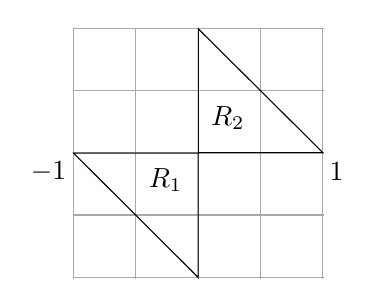
\begin{tikzpicture}[x=0.75pt,y=0.75pt,yscale=-1,xscale=1]
            %Shape: Grid [id:dp8044758903954956] 
            \draw  [draw opacity=0] (252.83,80.33) -- (373.67,80.33) -- (373.67,201.33) -- (252.83,201.33) -- cycle ; \draw  [color={rgb, 255:red, 168; green, 168; blue, 168 }  ,draw opacity=1 ] (252.83,80.33) -- (252.83,201.33)(282.83,80.33) -- (282.83,201.33)(312.83,80.33) -- (312.83,201.33)(342.83,80.33) -- (342.83,201.33)(372.83,80.33) -- (372.83,201.33) ; \draw  [color={rgb, 255:red, 168; green, 168; blue, 168 }  ,draw opacity=1 ] (252.83,80.33) -- (373.67,80.33)(252.83,110.33) -- (373.67,110.33)(252.83,140.33) -- (373.67,140.33)(252.83,170.33) -- (373.67,170.33)(252.83,200.33) -- (373.67,200.33) ; \draw  [color={rgb, 255:red, 168; green, 168; blue, 168 }  ,draw opacity=1 ]  ;
            %Shape: Right Triangle [id:dp6090851976145147] 
            \draw   (313,80.67) -- (373,140.33) -- (313,140.33) -- cycle ;
            %Shape: Right Triangle [id:dp2511359111159521] 
            \draw   (312.83,200.33) -- (252.83,140.5) -- (312.83,140.5) -- cycle ;

            % Text Node
            \draw (375,143.73) node [anchor=north west][inner sep=0.75pt]    {$1$};
            % Text Node
            \draw (231,143.4) node [anchor=north west][inner sep=0.75pt]    {$-1$};
            % Text Node
            \draw (287.83,146.73) node [anchor=north west][inner sep=0.75pt]    {$R_{1}$};
            % Text Node
            \draw (317.83,116.73) node [anchor=north west][inner sep=0.75pt]    {$R_{2}$};
        \end{tikzpicture}
    \end{figure}
\end{Example}

\begin{Remark}{}{}
    If we are lucky, we can use geometric formulas to evaluate integrals
    (see pg 26--28 in the notes). However, we are almost never this lucky\textellipsis{}
\end{Remark}

\section{Average Value of a Function}

\begin{Definition}{Average value}{avg_value}
    If $ f $ is continuous on $ \interval{a}{b} $, the \textbf{average value} of $ f $
    on $ \interval{a}{b} $ is defined as
    $ \displaystyle \frac{1}{b-a} \int_{a}^{b} f(x)\,dx $.
\end{Definition}

\subsection*{Geometric Interpretation}
\begin{Proof}{\ref{thm:avt}}{}
    If $ f $ is continuous on $ \interval{a}{b} $, EVT says there exists $ m,M\in\mathbb{R} $ such that
    $ \displaystyle m\le f(x) \le M $
    for $ x\in\interval{a}{b} $, and $ f(c_1)=m $, $ f(c_2)=M $ for some $ c_1,c_2\in\interval{a}{b} $.

    Also, we know
    \begin{align*}
        m(b-a)\le \int_{a}^{b} f(x)\, d{x} \le M(b-a)
         & \implies m\le \frac{1}{b-a} \int_{a}^{b} f(x)\, d{x} \le M       \\
         & \iff f(c_1)\le \frac{1}{b-a} \int_{a}^{b} f(x)\, d{x} \le f(c_2) \\
    \end{align*}
    IVT says there exists $ c $ between $ c_1 $ and $ c_2 $, so that
    \[ f(c)=\frac{1}{b-a} \int_{a}^{b} f(x)\, d{x} \]
\end{Proof}

\begin{Theorem}{Average Value Theorem (AVT)}{avt}
    Assume $ f $ is continuous on $ \interval{a}{b} $.
    There exists $ c\in\interval{a}{b} $ such that
    $ \displaystyle f(c)=\frac{1}{b-a} \int_{a}^{b} f(x) d{x} $.
\end{Theorem}

\begin{Remark}{}{}
    Note that this theorem holds even if $ b<a $ since
    \begin{align*}
        f(c) & =\frac{1}{a-b} \int_{b}^{a}\, f(x)dx                  \\
             & =\frac{1}{a-b}\biggl(-\int_{a}^{b} f(x)\, d{x}\biggr) \\
             & =\frac{1}{b-a} \int_{a}^{b} f(x)\, d{x}
    \end{align*}
\end{Remark}

The big problem we face now is that evaluating $ \int_{a}^{b} f(x)\, d{x} $ is
monstrously difficult for all but the simplest of functions.

IF ONLY THERE WAS A BETTER WAY\@!

(spoilers: there's a better way! It's the Fundamental Theorem of Calculus!)


\makeheading{Week 2}{\daterange{2021-09-13}{2021-09-17}}%chktex 8
\section{Module 1: Measures of Disease Frequency}
\subsection{Incidence and Prevalence Rates}
\subsubsection*{How do we measure and evaluate patterns of disease within a population?}
\begin{figure}[H]
    \centering
    \includegraphics[width=0.75\textwidth]{1.1/1.pdf}
\end{figure}
\subsubsection*{Primer on HIV/AIDS}
\begin{itemize}
    \item HIV (human immunodeficiency virus) is a virus that attack’s the body’s immune
          system.
    \item HIV is spread through sexual contact, sharing needles, and mother-to-child
          transmission during pregnancy, childbirth, or breastfeeding.
    \item Infection with HIV can lead to AIDS (acquired immunodeficiency syndrome).
    \item Individuals with AIDS are at increased risk of infection and infection-related
          cancers.
    \item Currently, no cure exists, but antiretroviral therapy can slow the progression of the
          disease.
\end{itemize}
\subsubsection*{1.1 Incidence and Prevalence Rates}
\begin{Regular}
    \textcolor{Blue}{Goal}: How do we measure and evaluate patterns of disease within a population?
\end{Regular}
\begin{itemize}
    \item \textcolor{Blue}{Prevalence}: The proportion of the population currently affected by a disease.
    \item \textcolor{Blue}{Incidence}: The rate at which new cases of a disease develop in a population.
\end{itemize}
\subsubsection*{Number of people living with HIV/AIDS 1990--2017}
\begin{figure}[H]
    \centering
    \includegraphics[width=0.75\textwidth]{1.1/2.pdf}
\end{figure}
\subsubsection*{Prevalence}
\textcolor{Blue}{Prevalence}: The proportion of the population currently affected by a disease.
\begin{Regular}
    \[ \begin{tabular}{>{\bfseries}c}
            Point Prevalence \\
            per 1000
        \end{tabular}=\frac{\begin{tabular}{>{\bfseries}c}
                Number of cases (new and pre-existing) in the \\
                population at a fixed point in time
            \end{tabular}}{\begin{tabular}{>{\bfseries}c}
                Number of individuals in the \\
                population at a fixed point in time
            \end{tabular}}\times 1000.  \]
\end{Regular}
\begin{Regular}
    \[ \begin{tabular}{>{\bfseries}c}
            Period Prevalence \\
            per 1000
        \end{tabular}=\frac{\begin{tabular}{>{\bfseries}c}
                Number of cases (new and pre-existing) in the \\
                population over a given time period
            \end{tabular}}{\begin{tabular}{>{\bfseries}c}
                Number of individuals in the \\
                population over a given time period
            \end{tabular}}\times 1000.  \]
\end{Regular}
\subsubsection*{Prevalence of HIV/AIDS 1990--2017}
\begin{figure}[H]
    \centering
    \includegraphics[width=0.75\textwidth]{1.1/3.pdf}
\end{figure}
\subsubsection*{Annual new cases of HIV infection, 1990--2017}
\begin{figure}[H]
    \centering
    \includegraphics[width=0.75\textwidth]{1.1/4.pdf}
\end{figure}
\subsubsection*{Cumulative Incidence}
\textcolor{Blue}{Incidence}: The rate at which \textbf{new cases} of a disease develop in a \textbf{population} over a
specific \textbf{time} period.
\begin{Regular}
    \[ \begin{tabular}{>{\bfseries}c}
            Cumulative Incidence \\
            per 1000
        \end{tabular}=\frac{\begin{tabular}{>{\bfseries}c}
                Number of new cases in the \\
                population over the time period of interest
            \end{tabular}}{\begin{tabular}{>{\bfseries}c}
                Number of individuals at risk in the \\
                population at the start of the time period of interest
            \end{tabular}}\times 1000.  \]
\end{Regular}
\begin{itemize}
    \item Assumes all subjects remain in the population and at risk for the entire time period.
    \item Easily violated: Births, deaths, immigration, emigration, case diagnosis.
    \item Consider two ways to refine the denominator calculation.
          \begin{enumerate}[1.]
              \item Use a mid-interval population estimate.
              \item Calculate the total person-time at risk in the population.
          \end{enumerate}
\end{itemize}
\subsubsection*{Incidence Density or Incidence Rate}
\begin{Regular}
    \[ \begin{tabular}{>{\bfseries}c}
            Incidence Density \\
            per 1000
        \end{tabular}=\frac{\begin{tabular}{>{\bfseries}c}
                Number of new cases in the \\
                population over the time period of interest
            \end{tabular}}{\begin{tabular}{>{\bfseries}c}
                Mid-interval estimate of the population
            \end{tabular}}\times 1000.  \]
\end{Regular}
\begin{Example}
    \begin{itemize}
        \item 3,218 new cases of HIV in Canada, 2016.
        \item 36,264,604 July 1, 2016 Canadian population estimate.
              \[ \begin{tabular}{>{\bfseries}c}
                      Incidence Density \\
                      per 100,000
                  \end{tabular}=\frac{3,218}{36,264,604}\times 100,000=8.873666. \]
        \item \emph{The incidence of HIV infection in Canada in the year 2016 was 8.87 cases per
                  100,000 persons}.
    \end{itemize}
\end{Example}
\subsubsection*{Incidence of HIV per 1,000 uninfected adults, 2000--2017}
\begin{figure}[H]
    \centering
    \includegraphics[width=0.75\textwidth]{1.1/5.pdf}
\end{figure}
\subsubsection*{Person-time at risk}
\begin{itemize}
    \item To account for varying time periods of risk we consider an alternative denominator
          for our incidence calculation.
    \item Person-time at risk is the duration of time an individual is at risk for developing
          a disease.
    \item Assuming they are initially disease free, it is the length of time from baseline until
          the first of:
          \begin{enumerate}[1.]
              \item They develop the disease of interest and become a case.
              \item They cease to be at risk of becoming a case due to either death from unrelated
                    causes or they leave the population.
              \item The end of the time period of interest is reached.
          \end{enumerate}
    \item Total person-time at risk is the sum of the individual contributions over the
          population.
\end{itemize}
\subsubsection*{Incidence Density or Incidence Rate}
\begin{Regular}
    \[ \begin{tabular}{>{\bfseries}c}
            Incidence Density \\
            per 1000
        \end{tabular}=\frac{\begin{tabular}{>{\bfseries}c}
                Number of new cases in the \\
                population over the time period of interest
            \end{tabular}}{\begin{tabular}{>{\bfseries}c}
                Mid-Total person-time at risk in the \\
                population over the time period of interest
            \end{tabular}}\times 1000.  \]
\end{Regular}
\begin{itemize}
    \item Incidence density estimate is more precise than cumulative incidence, but may be
          harder to get information needed, so this measure is often used for small
          populations.
    \item Expressed as per $10^x$ person-years (-month, -day).
\end{itemize}
\subsubsection*{Relationship Between Incidence and Prevalence}
\begin{figure}[H]
    \centering
    \includegraphics[width=0.25\textwidth]{1.1/6.jpg}
\end{figure}
\subsubsection*{Relationship Between Incidence and Prevalence}
\begin{itemize}
    \item \textbf{Incidence}: the rate new cases are diagnosed in a population.
    \item \textbf{Prevalence}: the proportion of the population currently affected by the disease.
\end{itemize}
\begin{Regular}
    \[ \textbf{Prevalence}\approx \textbf{Incidence}\times \textbf{Disease Duration} \]
\end{Regular}
\begin{itemize}
    \item Relationship is approximate but generally holds well if prevalence is low ($<10\,$\%)
          and duration is fairly constant (or an average can be taken).
    \item Note: units must be consistent in order to perform the multiplication operation.
\end{itemize}
\subsubsection*{Prevalence, new cases, and mortality for HIV/AIDS}
\begin{figure}[H]
    \centering
    \includegraphics[width=0.75\textwidth]{1.1/7.pdf}
\end{figure}
\subsubsection*{Exercise: Incidence and Prevalence Calculations}
Total population size of 100. Histories of 12 subjects with disease are below. Subjects
13--100 do not have the disease during the year of study. ($ \triangle $ Diagnosis; $ \times $ Death)
\begin{table}[H]
    \centering
    \begin{tabular}{ccc}
        \toprule
        \textbf{Subject} & \textbf{Diagnosis} $ \triangle $ & \textbf{Death} $ \times $ \\
        \midrule
        1                & $<$ January 1                                                \\
        2                & $<$ January 1                    & April 30                  \\
        3                & $<$ January 1                                                \\
        4                & $<$ January 1                                                \\
        5                & $<$ January 1                    & June 30                   \\
        6                & March 1                          & October 31                \\
        7                & May 1                                                        \\
        8                & May 1                                                        \\
        9                & July 1                                                       \\
        10               & July 1                           & October 31                \\
        11               & NA                               & May 1                     \\
        12               & NA                               & September 1               \\
        13--100          & NA                                                           \\
        \bottomrule
    \end{tabular}
\end{table}
\begin{figure}[H]
    \centering
    \includegraphics[width=0.75\textwidth]{1.1/8.pdf}
\end{figure}
\begin{itemize}
    \item Point Prevalence on July 1.
    \item Period Prevalence (Jan 1 to Dec 31)
    \item Cumulative Incidence (Jan 1 to Dec 31).
    \item Incidence Density (Jan 1 to Dec 31).
\end{itemize}
\begin{align*}
    \begin{tabular}{c}
        Point Prevalence \\
        on July 1
    \end{tabular}
     & =\frac{\text{\# cases in the pop on July 1}}{\text{\# indv in the pop on July 1}}\times 1000=\frac{8}{97}\times 1000=\text{$82.47$ per 1000 persons}.                     \\\\
    \begin{tabular}{c}
        Period Prevalence \\
        (Jan 1-Dec 31)
    \end{tabular}
     & =\frac{\text{\# cases during Jan 1-Dec 31}}{\text{\# indv in the pop Jan 1-Dec 31}}\times 1000=\frac{10}{100}\times 1000=\text{$100$ per 1000 persons}.                   \\\\
    \begin{tabular}{c}
        Cumulative Incidence \\
        (Jan 1-Dec 31)
    \end{tabular}
     & =\frac{\text{\# new cases during Jan 1-Dec 31}}{\text{\# indv at risk on Jan 1}}\times 1000=\frac{5}{95}\times 1000=\text{$52.63$ per 1000 persons}.                      \\\\
    \begin{tabular}{c}
        Incidence Density \\
        (Jan 1-Dec 31)
    \end{tabular}
     & =\frac{\text{\# new cases during Jan 1-Dec 31}}{\text{July 1 population size}}\times 1000=\frac{5}{97}\times 1000=\text{$51.55$ per 1000 persons}.                        \\\\
    \begin{tabular}{c}
        Incidence Density \\
        (Jan 1-Dec 31)
    \end{tabular}
     & =\frac{\text{\# new cases during Jan 1-Dec 31}}{\text{\small Total person-years at risk Jan 1-Dec 31}}\times 1000=\frac{5}{90.83}\times 1000=\text{$55.05$ per 1000 p-y}. \\
\end{align*}
\subsection{Standardization of Rates: Indirect Methods}
% Chapter 2 Part 1
\chapter{Causal Inference and Potential Outcomes}
\makeheading{Week 3}{\daterange{2022-01-17}{2022-01-21}}%chktex 8
\section{Causal Inference}
\subsection{Introduction}
\subsubsection{Reference}
\begin{itemize}
    \item Hernán M.A., \& Robins J.M. (2020). Causal Inference: What
          If. Boca Raton: Chapman Hall/CRC\@.

          \url{https://www.hsph.harvard.edu/miguel-hernan/
              causal-inference-book/}
\end{itemize}
\subsubsection{Causal Inference}
Two notions of causation:
\begin{itemize}
    \item Causes of an effect/outcome.
    \item Effects of a cause.
\end{itemize}
\textbf{Causes of an effect}
\begin{itemize}
    \item What are causes of lung cancer?
    \item What was the cause of outbreak of food poisoning?
\end{itemize}
\textbf{Effects of a cause/intervention}
\begin{itemize}
    \item Does smoking cause lung cancer?
    \item Does mixed feeding cause obesity?
    \item How strong is the effect?
\end{itemize}
\begin{itemize}
    \item We concentrate on effects of a cause/treatment/intervention.
    \item Fundamentally simpler question: search is for useful
          information rather than complete scientific understanding.
    \item Typical approach for estimating causal effects (which may be
          problematic):
          collect sample on treatments/exposures, outcomes, and other
          variables in population; Use standard statistical methods
          (such as multiple regression) to derive inferences about
          associations between observable variables.
\end{itemize}
\subsubsection*{A Note}
\begin{itemize}
    \item In pharmaceutical companies, people used to believe
          conducting randomized clinical trials is the only way to
          evaluate a newly developed drug. However, there is a shifting
          trend going on right now because of:
          \begin{itemize}
              \item Difficult to find control subjects.
              \item Compliance issue.
              \item Exclusion criteria.
              \item Cost issue.
          \end{itemize}
    \item New trend: utilizing existing Electronic Health Records data
          to help find controls.
    \item The study is not randomized any more: observational study.
\end{itemize}
\subsubsection*{Draw Causality}
\textbf{Observational Studies}
\begin{itemize}
    \item No control over which subjects have the exposure and which
          do not.
    \item Exposed and Unexposed groups may be quite different with
          respect to other subject characteristics
    \item It is sometimes useful to use these studies to look at the
          natural history of a disease, but any attempt to identify
          causality b/t a risk factor and outcome must be done w/
          great caution.
\end{itemize}
\subsection{Confounding}
\subsubsection*{Confounding Issue in Observational Studies}
\begin{Example}{}
    Differences in the outcome are not only due to the treatment, but
    also because of the masking effect of covariates (confounders).
    \begin{center}
        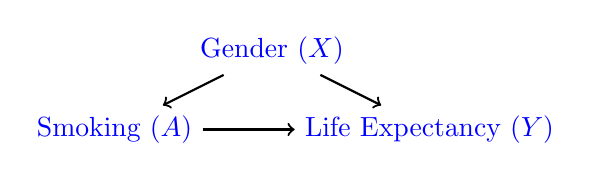
\begin{tikzpicture}[thick]
            \node (1) at (0,1) {\textcolor{Blue}{Gender ($ X $)}};
            \node (2) at (-2,0) {\textcolor{Blue}{Smoking ($ A $)}};
            \node (3) at (2,0) {\textcolor{Blue}{Life Expectancy ($ Y $)}};
            \draw[->] (1) to (2);
            \draw[->] (1) to (3);
            \draw[->] (2) to (3);
        \end{tikzpicture}
    \end{center}
    Here, gender is known as a confounder. Very often, in real
    applications, the list of potential confounders could be very large,
    and even high-dimensional.
\end{Example}
\subsubsection*{Another Example of Confounding}
\begin{Example}{}
    Researchers find when the consumption of ice cream increases, the
    death from drowning increases. Does eating ice cream lead to
    drowning?
    \begin{center}
        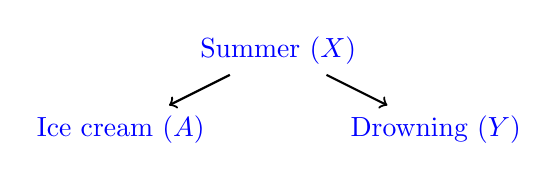
\begin{tikzpicture}[thick]
            \node (1) at (0,1) {\textcolor{Blue}{Summer ($ X $)}};
            \node (2) at (-2,0) {\textcolor{Blue}{Ice cream ($ A $)}};
            \node (3) at (2,0) {\textcolor{Blue}{Drowning ($ Y $)}};
            \draw[->] (1) to (2);
            \draw[->] (1) to (3);
        \end{tikzpicture}
    \end{center}
    Here, summer (hot weather) is a confounder.
\end{Example}
\subsubsection*{Potential Outcomes Framework}
\begin{itemize}
    \item Useful to have more precise definitions of causal effects.
    \item Demystifies the process of going from association to causation.
    \item Allows explicit statements regarding what assumptions are
          necessary to justify causal inferences.
    \item Allows for more critical, better informed evaluation of causal
          claims.
    \item Helps determine when familiar methods useful or unfamiliar
          methods necessary.
    \item Motivates derivation and use of unfamiliar methods.
\end{itemize}
\section{Potential Outcomes Framework}
\subsection*{Definition of a Causal Effect}
\begin{Regular}{}
    Suppose we have data on subjects $ i=1,\ldots,n $.
    \begin{itemize}
        \item $ \Vector{X}_i=(\Vector{X}_{i1},\Vector{X}_{i2},\ldots,\Vector{X}_{ip})^\top $: baseline covariates/potential confounders.
        \item $ A_i $: treatment assignment/exposure status for subject $ i $
              \[ A_i=\begin{cases*}
                      1, & if exposed/treated,   \\
                      0, & if unexposed/treated.
                  \end{cases*} \]
        \item $ Y_i $: observed outcome for subject $ i $.
    \end{itemize}
    \textbf{Counterfactuals/Potential outcomes}
    \begin{itemize}
        \item $ Y_i^1 $: the potential outcome if subject $ i $ were \textcolor{Blue}{treated/exposed}.
        \item $ Y_i^0 $: the potential outcome if subject $ i $ were \textcolor{Blue}{untreated/unexposed}.
    \end{itemize}
\end{Regular}
\begin{Regular}{}
    The \textbf{individual-level causal effect} for subject $ i $ is:
    \[ Y_i^1-Y_i^0. \]
\end{Regular}
\begin{Regular}{Causal Estimand}
    The \textbf{average causal effect} (ACE) is:
    \[ \ACE=\E{Y_i^1-Y_i^0}=\E{Y_i^1}-\E{Y_i^0}, \]
    where
    \begin{itemize}
        \item $ \E{Y_i^1} $ is the mean potential outcome had all subjects in the population
              were treated/exposed, and
        \item $ \E{Y_i^0} $ is the mean potential outcome had all subjects in the population were untreated/unexposed.
    \end{itemize}
    \tcblower{}
    If $ Y $ is binary,
    \begin{itemize}
        \item ACE is causal excess risk (omit subscript $ i $):
              \[ \E{Y^1-Y^0}=\E{Y^1}-\E{Y^0}=\Prob{Y^1=1}-\Prob{Y^0=1}. \]
        \item \textbf{Causal relative risk}:
              \[ \frac{\Prob{Y^1=1}}{\Prob{Y^0=1}}. \]
        \item \textbf{Causal odds ratio}:
              \[ \frac{\Prob{Y^1=1}/\Prob{Y^1=0}}{\Prob{Y^0=1}/\Prob{Y^0=0}}. \]
        \item \textbf{Crude excess risk}:
              \[ \Prob{Y=1\given A=1}-\Prob{Y=1\given A=0}. \]
        \item \textbf{Crude relative risk}:
              \[ \frac{\Prob{Y=1\given A=1}}{\Prob{Y=1\given A=0}}. \]
        \item \textbf{Crude odds ratio}:
              \[ \frac{\Prob{Y=1\given A=1}/\Prob{Y=0\given A=1}}{\Prob{Y=1\given A=0}/\Prob{Y=0\given A=0}}. \]
    \end{itemize}
\end{Regular}
\subsection*{A Toy Example}
\begin{Example}{}
    Assume we have a population of 8 subjects:
    \[ \begin{array}{cccc}
                  & A & Y^0 & Y^1 \\
            \midrule
            S_{1} & 0 & 0   & 1   \\
            S_{2} & 0 & 1   & 1   \\
            S_{3} & 0 & 0   & 0   \\
            S_{4} & 0 & 0   & 0   \\
            S_{5} & 1 & 0   & 0   \\
            S_{6} & 1 & 1   & 0   \\
            S_{7} & 1 & 1   & 1   \\
            S_{8} & 1 & 0   & 1   \\
            \bottomrule
        \end{array} \]
    We get
    \[ \text{Causal excess risk (ACE)} =\Prob{Y^1=1}-\Prob{Y^0=1}=\frac{4}{8}-\frac{3}{8}=\frac{1}{8}. \]
    For crude excess risk, we have
    \[ \begin{array}{ccccc}
                  & A & Y^0 & Y^1 & Y \\
            \midrule
            S_{1} & 0 & 0   & 1   & 0 \\
            S_{2} & 0 & 1   & 1   & 1 \\
            S_{3} & 0 & 0   & 0   & 0 \\
            S_{4} & 0 & 0   & 0   & 0 \\
            S_{5} & 1 & 0   & 0   & 0 \\
            S_{6} & 1 & 1   & 0   & 0 \\
            S_{7} & 1 & 1   & 1   & 1 \\
            S_{8} & 1 & 0   & 1   & 1 \\
            \bottomrule
        \end{array} \]
    \[ \text{Crude excess risk}=\Prob{Y=1\given A=1}-\Prob{Y=1\given A=0}=\frac{2}{4}-\frac{1}{4}=\frac{1}{4}. \]
\end{Example}
\subsection*{Fundamental Problem of Causal Inference}
\begin{Regular}{}
    For subject $ i $, we only get to observe one of $ Y_i^1 $ and $ Y_i^0 $, that is,
    \[ Y_i=Y_i^1A_i+Y_i^0(1-A_i). \]
    \tcblower{}
    \underline{Remarks}:
    \begin{enumerate}[(1)]
        \item In the literature, the above equality is often referred as the
              consistency assumption for causal inference
        \item For each subject $i$, one of the two potential outcomes is
              always missing.
        \item For this reason, many people believe causal inference is
              essentially a missing data problem.
    \end{enumerate}
\end{Regular}
\section{Estimation}
\begin{Regular}{}
    In \textbf{randomized studies}:
    \begin{itemize}
        \item $ \E{Y\given A=1}=\E{Y^1\given A=1}=\E{Y^1} $, and
        \item $ \E{Y\given A=0}=\E{Y^0\given A=0}=\E{Y^0} $.
    \end{itemize}
    Consequently, an unbiased estimate of ACE is:
    \begin{align*}
        \widehat{\ACE}
         & =\estE{Y^1}-\estE{Y^0}                                                                                   \\
         & =\estE{Y\given A=1}-\estE{Y\given A=0}                                                                   \\
         & =\frac{\sum_{i=1}^{n}Y_i A_i}{\sum_{i=1}^{n}A_i}-\frac{\sum_{i=1}^{n}Y_i(1-A_i)}{\sum_{i=1}^{n}(1-A_i)},
    \end{align*}
    where
    \begin{itemize}
        \item $ \sum_{i=1}^{n}A_i=n_1 $ is the number of treated/exposed subjects in the sample, and
        \item $ \sum_{i=1}^{n}(1-A_i)=n_0 $ is the number of untreated/unexposed subjects in the sample.
    \end{itemize}
\end{Regular}
\begin{Regular}{}
    In \textbf{observational studies}:
    \begin{itemize}
        \item $ \E{Y\given A=1}=\E{Y^1\given A=1}\ne\E{Y^1} $, and
        \item $ \E{Y\given A=0}=\E{Y^0\given A=0}\ne\E{Y^0} $,
    \end{itemize}
    where the inequalities are due to selection bias.
    Therefore, the estimator in randomized studies is biased for ACE in
    observational studies.
\end{Regular}
\section*{Assumptions for Causal Inference}
\section{Assumption 1}
\begin{Regular}{Assumption 1: Strongly Ignorable Treatment Assignment (SITA)}
    \[ (Y^0,Y^1)\indep (A\mid X). \]
    \tcblower{}
    \underline{Remarks}:
    \begin{itemize}
        \item In observational studies, it means $X$ includes all possible
              confounders (no unmeasured confounders).
        \item In randomized studies, we have $ (Y^0,Y^1)\indep A $.
        \item Within a subset of subjects with similar $X$, exposure/treatment
              can be viewed as if it were randomly assigned.
        \item This assumption cannot be verified on the observed data;
              more plausible as the size of $X$ grows.
        \item If violated, instrumental variable approach can be used in
              some cases.
    \end{itemize}
\end{Regular}
\section{Assumptions 2--4}
\begin{Regular}{Assumption 2: Stable Unit Treatment Value Assumption (SUTVA)}
    \[ (Y_i^0,Y_i^1)\indep A_j\text{ for $i\ne j$}. \]
    \tcblower{}
    \underline{Remarks}:
    \begin{itemize}
        \item Each subject's potential outcomes are not influenced by the
              actual treatment status of other subjects.
        \item Counter-example: infectious disease, family studies.
        \item If violated, divide the subjects into clusters.
    \end{itemize}
\end{Regular}
\begin{Regular}{Assumption 3: Common Support Condition (CSC)}
    \[ 0<\Prob{A=1\given X=x}<1\text{ for any $x$}. \]
    \tcblower{}
    \underline{Remarks}:
    \begin{itemize}
        \item It means that $ Y^0 $ and $ Y^1 $ should both exist in principle.
        \item Can be violated if a particular group of subjects in the
              population always receive the treatment or never receive the
              treatment.
        \item If violated, re-define the population (exclude those subjects).
    \end{itemize}
\end{Regular}
\begin{Regular}{Assumption 4: Consistency}
    \[ Y=Y^1 A+Y^0(1-A). \]
    \tcblower{}
    \underline{Remarks}:
    \begin{itemize}
        \item The observed outcome for a subject equals to the potential
              outcome under the actual treatment assignment the subject
              receives.
        \item Can be violated if different versions of treatment have
              different causal effects.
    \end{itemize}
\end{Regular}
\section{Propensity Scores}
\subsection*{Motivation for Propensity Scores}
The SITA assumption $(Y^0,Y^1)\indep (A\mid X)$ gives us some ideas about how to
estimate causal effects for observational studies.
\begin{itemize}
    \item If we condition on $X$, we can estimate the causal effect as in a
          randomized study, which is relatively straightforward.
    \item  However, if $X$ contains a large number of covariates,
          conditioning on $X$ is challenging (curse of dimensionality).
    \item  Solution: propensity score methods
\end{itemize}
\begin{Regular}{}
    \textbf{Propensity score} is the conditional probability of being exposed/treated given baseline covariates:
    \[ \ps{x}=\Prob{A=1\given X=x}. \]
    Also,
    \[ \ps{X}=\Prob{A=1\given X}. \]
    \tcblower{}
    \underline{Remarks}:
    \begin{itemize}
        \item In simple randomized studies, $ \ps{x}=0.5 $.
        \item In observational studies, $ \ps{x} $ is unknown and must be estimated.
    \end{itemize}
\end{Regular}
\subsection*{Properties}
\subsubsection*{Properties of Propensity Score}
\begin{itemize}
    \item Propensity score is a balancing score:
          \[ X\indep (A\mid \ps{X}) \]
    \item If the treatment is strongly ignorable given $ X $, that is,
          \[ (Y^0,Y^1)\indep (A\mid X), \]
          then it is strongly ignorable given $ \ps{x} $
          \[ (Y^0,Y^1)\indep (A\mid \ps{X}). \]
    \item $ \ps{x} $ is a scalar, free of dimension of $ X $.
    \item It is a summary of the contribution of all baseline characteristics to the exposure/treatment assignment.
\end{itemize}
\section{Properties of Propensity Score}
\begin{Result}{}
    The propensity score is a \textbf{balancing score}, that is,
    \[ X\indep(A\mid \ps{X}) \]
    \tcblower{}
    \textbf{Proof}: Rosenbaum and Rubin (1983).
    \begin{align*}
        \Prob[\big]{A=1\given \ps{X},X}
         & =\Prob{A=1\given X} &  & \text{$\ps{X}$ is a function of $X$} \\
         & =\ps{X}.
    \end{align*}
    On the other hand,
    \begin{align*}
        \Prob[\big]{A=1\given \ps{X}}
         & =\E[\big]{A\given \ps{X}}                                                  &  & \text{since $A$ is binary}    \\
         & =\E[\big]{\E{A\given \underbrace{X}_{C_1}}\given\underbrace{\ps{X}}_{C_2}} &  & \text{LIE since $C_2=f(C_1)$} \\
         & =\E[\big]{\ps{X}\given \ps{X}}                                                                                \\
         & =\ps{X}.
    \end{align*}
    Therefore,
    \[ \Prob[\big]{A=1\given \ps{X},X}=\Prob[\big]{A=1\given \ps{X}}. \]
    In other words, $ X\indep (A\mid \ps{X}) $.
\end{Result}
\begin{Result}{}
    If $ (Y^0,Y^1)\indep (A\mid X) $, then
    \[ (Y^0,Y^1)\indep(A\mid \ps{X}). \]
    \tcblower{}
    \textbf{Proof}:
    \begin{align*}
        \Prob{A=1\given Y^0,Y^1,\ps{X}}
         & =\E{A\given Y^0,Y^1,\ps{X}}                                                                 &  & \text{since $A$ is binary}      \\
         & =\E[\big]{\E{A\given \underbrace{Y^0,Y^1,X}_{C_1}}\given \underbrace{Y^0,Y^1,\ps{X}}_{C_2}} &  & \text{LIE since $C_2=f(C_1)$}   \\
         & =\E[\big]{\E{A\given X}\given Y^0,Y^1,\ps{X}}                                               &  & \text{SITA}                     \\
         & =\E[\big]{\ps{X}\given Y^0,Y^1,\ps{X}}                                                                                           \\
         & =\ps{X}                                                                                                                          \\
         & =\Prob[\big]{A=1\given \ps{X}}.                                                             &  & \text{from the previous result}
    \end{align*}
    Therefore,
    \[ (Y^0,Y^1)\indep(A\mid \ps{X}). \]
\end{Result}
\chapter{ARIMA Models Continued}
\section{Stationary Process Forecasting}
Suppose we observe a time series
$ X_1,\ldots,X_T $
that we believe has been generated by an underlying
stationary process. We would like to
produce an $ h $-step ahead
forecast
\[ \hat{X}_{T+h}=\hat{X}_{T+h\mid T}=f(X_t,\ldots,X_1) \]
forecasting $ X_{T+h} $. Ideally, $ \hat{X}_{T+h} $
would minimize the prediction error
\[ L(X_{T+h},\hat{X}_{T+h})=\min_f
    L(X_{T+h},f(X_{T},\ldots,X_1)) \]
where $ L $ is a loss function.

Frequently, the loss function is taken
to be the \emph{mean-squared error} (MSE)
\[ L(X_{T+h},\hat{X}_{T+h})=
    \E[\big]{(X_{T+h}-\hat{X}_{T+h})^2} \]
When using MSE, it is natural to consider
\[ L^2=\set{\text{Random variables } X: \E{X^2}<\infty} \]
$ L^2 $ is a Hilbert space when equipped
with the inner product
\[ \innerp{X}{Y}=\E{XY} \]
Hilbert spaces are generalizations of Euclidean space ($ \mathbf{R}^d $)
in which the geometry and notation of projection
are preserved.
\[ \text{Proj}(X\to Y)=\innerp{X}{Y}Y \]
\begin{Theorem}{Projection Theoren}{}
    We say $ M\subseteq L^2 $
    is a \textbf{closed linear subspace}, if
    \begin{itemize}
        \item Linearity: $ X,Y\in M $, $ \alpha,\beta\in\mathbf{R} $
              then $ \alpha X+\beta Y\in M $
        \item Closed: If $ X_n\to X $ ($ \E{(X_n-X)^2} $),
              and $ X_n\in M $, then $ X\in M $.
    \end{itemize}
    If $ M $ is a closed linear subspace in $ L^2 $
    and $ x\in L^2 $, then there exists a
    unique $ \hat{X}\in M $ such that
    \[ \E{(X-\hat{X})^2}=\inf_{y\in M}\E{(X-Y)^2} \]
    Moreover, $ \hat{X} $ satisfies the prediction equations/normal
    equations:
    \[ (X-\hat{X})\in M^\perp \implies \E{(X-\hat{X})Y}=0\quad (\forall y\in M) \]
\end{Theorem}
In MSE forecasting, we want to choose
$ \hat{X}_{T+h} $ satisfying
\[ \E{(X_{T+h}-\hat{X}_{T+h})^2}=\inf_{y\in M}\E{(X_{T+h}-y)^2} \]
where $ M $ is a closed linear subspace based on the available
data.
\begin{enumerate}[(1)]
    \item $ M=M_1=\set{z:z=f(X_{T},\ldots,X_{1}), f\text{ is any
                  Borel Measurable function}} $
          In this case
          \[ \hat{X}_{T+h}=\E{X_{T+h}\mid X_{T},\ldots,X_1} \]
          Unfortunately $ M_1 $ is enormous and complicated!
    \item $ M=M_2=\Span{1,X_{T},\ldots,X_1}=
              \set{Y:Y=\alpha_0+\sum_{j=1}^{T} \alpha_j X_j,\,\alpha_0,\ldots,\alpha_T\in\mathbf{R}} $
          which is the linear functions of $ X_1,\ldots,X_T $
          $ \hat{X}_{T+h} $ is called the \textbf{best linear predictor} (BLP).
\end{enumerate}


\subsection*{Example: Homelessness and Physical Health}
Data Source: Kleinman, K and Horton, NJ. SAS and R: \emph{Data
      Management, Statistical Analysis, and Graphics}. CRC Press.

The HELP (Health Evaluation and Linkage to Primary Care) study
was a clinical trial for adult patients recruited from a detoxification
unit. Patients with no primary care physician were randomized to
receive a multidisciplinary assessment and a brief motivational
intervention or usual care, with the goal of linking them to primary
medical care.

\textbf{Secondary Analysis}: Does homelessness affect physical health?
\url{http://sas-and-r.blogspot.com/2010/04/example-734-propensity-scores-and.html}

Available data:
\begin{itemize}
      \item \texttt{pcs}: measure of physical health via 36 question questionnaire
            (mean $48.05$, range $[14.07, 74.81]$).
      \item \texttt{homeless}: binary indicator of homelessness ($46.14\%$ homeless).
      \item \texttt{age}: in years (mean $35.65$, range $[19.00, 60.00]$).
      \item \texttt{female}: indicator of female sex ($23.62\%$ female).
      \item \texttt{i1}: alcohol intake per day (mean $17.9$, median $13.0$, range $[0,142]$).
      \item \texttt{mcs}: mental component summary measure
            (mean $31.68$, range $[6.76, 62.18]$).
\end{itemize}
\begin{itemize}
      \item Linear model for the association between homelessness and
            physical health:
            %\begin{noindent}
\begin{knitrout}
\definecolor{shadecolor}{rgb}{0.969, 0.969, 0.969}\color{fgcolor}\begin{kframe}
\begin{alltt}
\hlstd{ds} \hlkwb{<-} \hlkwd{read.csv}\hlstd{(}\hlstr{"data/help.csv"}\hlstd{)}
\hlkwd{attach}\hlstd{(ds)}
\hlkwd{summary}\hlstd{(}\hlkwd{lm}\hlstd{(pcs} \hlopt{~} \hlstd{homeless))}
\end{alltt}
\begin{verbatim}

Call:
lm(formula = pcs ~ homeless)

Residuals:
    Min      1Q  Median      3Q     Max 
-34.927  -7.903   0.644   8.387  25.805 

Coefficients:
            Estimate Std. Error t value Pr(>|t|)    
(Intercept)   49.001      0.688  71.220   <2e-16 ***
homeless      -2.064      1.013  -2.038   0.0422 *  
---
Signif. codes:  0 '***' 0.001 '**' 0.01 '*' 0.05 '.' 0.1 ' ' 1

Residual standard error: 10.75 on 451 degrees of freedom
Multiple R-squared:  0.009123,	Adjusted R-squared:  0.006926 
F-statistic: 4.152 on 1 and 451 DF,  p-value: 0.04216
\end{verbatim}
\end{kframe}
\end{knitrout}
      %\end{noindent}
            Unadjusted analysis: significant association between homelessness
            and physical health.
\end{itemize}
\subsection{Estimation}
\begin{itemize}
      \item Fit a logistic model for the propensity score
            %\begin{noindent}
\begin{knitrout}
\definecolor{shadecolor}{rgb}{0.969, 0.969, 0.969}\color{fgcolor}\begin{kframe}
\begin{alltt}
\hlstd{glm1} \hlkwb{<-} \hlkwd{glm}\hlstd{(homeless} \hlopt{~} \hlstd{age} \hlopt{+} \hlkwd{factor}\hlstd{(female)} \hlopt{+} \hlstd{i1} \hlopt{+} \hlstd{mcs,} \hlkwc{family} \hlstd{= binomial)}
\hlstd{PS} \hlkwb{<-} \hlstd{glm1}\hlopt{$}\hlstd{fitted.values}
\hlkwd{summary}\hlstd{(glm1)}
\end{alltt}
\begin{verbatim}

Call:
glm(formula = homeless ~ age + factor(female) + i1 + mcs, family = binomial)

Deviance Residuals: 
    Min       1Q   Median       3Q      Max  
-1.7603  -1.0271  -0.8211   1.2039   1.6332  

Coefficients:
                 Estimate Std. Error z value Pr(>|z|)    
(Intercept)     -0.658259   0.518953  -1.268   0.2046    
age              0.013659   0.012965   1.054   0.2921    
factor(female)1 -0.454530   0.237011  -1.918   0.0551 .  
i1               0.024878   0.005782   4.303 1.68e-05 ***
mcs             -0.009983   0.007768  -1.285   0.1987    
---
Signif. codes:  0 '***' 0.001 '**' 0.01 '*' 0.05 '.' 0.1 ' ' 1

(Dispersion parameter for binomial family taken to be 1)

    Null deviance: 625.28  on 452  degrees of freedom
Residual deviance: 592.54  on 448  degrees of freedom
AIC: 602.54

Number of Fisher Scoring iterations: 4
\end{verbatim}
\end{kframe}
\end{knitrout}
      %\end{noindent}
      \item Which variables should be included in the PS model? Real
            confounders and variables that are predictive of the outcome.
            %\begin{noindent}
\begin{knitrout}
\definecolor{shadecolor}{rgb}{0.969, 0.969, 0.969}\color{fgcolor}\begin{kframe}
\begin{alltt}
\hlkwd{summary}\hlstd{(}\hlkwd{lm}\hlstd{(pcs} \hlopt{~} \hlstd{age))}\hlopt{$}\hlstd{coef}
\end{alltt}
\begin{verbatim}
              Estimate Std. Error   t value     Pr(>|t|)
(Intercept) 59.4549837 2.33874676 25.421728 4.125943e-89
age         -0.3199256 0.06411778 -4.989655 8.651612e-07
\end{verbatim}
\begin{alltt}
\hlkwd{summary}\hlstd{(}\hlkwd{lm}\hlstd{(pcs} \hlopt{~} \hlstd{female))}\hlopt{$}\hlstd{coef}
\end{alltt}
\begin{verbatim}
             Estimate Std. Error   t value      Pr(>|t|)
(Intercept) 48.986239  0.5732719 85.450274 1.076730e-280
female      -3.969879  1.1795541 -3.365576  8.291456e-04
\end{verbatim}
\begin{alltt}
\hlkwd{summary}\hlstd{(}\hlkwd{lm}\hlstd{(pcs} \hlopt{~} \hlstd{i1))}\hlopt{$}\hlstd{coef}
\end{alltt}
\begin{verbatim}
              Estimate Std. Error   t value      Pr(>|t|)
(Intercept) 49.9424609 0.66766179 74.802036 2.407295e-256
i1          -0.1057625 0.02487199 -4.252273  2.573816e-05
\end{verbatim}
\begin{alltt}
\hlkwd{summary}\hlstd{(}\hlkwd{lm}\hlstd{(pcs} \hlopt{~} \hlstd{mcs))}\hlopt{$}\hlstd{coef}
\end{alltt}
\begin{verbatim}
               Estimate Std. Error   t value      Pr(>|t|)
(Intercept) 45.10957488 1.34341383 33.578317 9.114672e-125
mcs          0.09278014 0.03931041  2.360192  1.869034e-02
\end{verbatim}
\end{kframe}
\end{knitrout}
      %\end{noindent}
      \item Check that there is a reasonable amount of overlap in the
            propensity scores between the two groups:
            %\begin{noindent}
\begin{knitrout}
\definecolor{shadecolor}{rgb}{0.969, 0.969, 0.969}\color{fgcolor}\begin{kframe}
\begin{alltt}
\hlkwd{summary}\hlstd{(PS[homeless} \hlopt{==} \hlnum{0}\hlstd{])}
\end{alltt}
\begin{verbatim}
   Min. 1st Qu.  Median    Mean 3rd Qu.    Max. 
 0.2137  0.3474  0.4040  0.4297  0.4980  0.7876 
\end{verbatim}
\begin{alltt}
\hlkwd{summary}\hlstd{(PS[homeless} \hlopt{==} \hlnum{1}\hlstd{])}
\end{alltt}
\begin{verbatim}
   Min. 1st Qu.  Median    Mean 3rd Qu.    Max. 
 0.2635  0.4003  0.4739  0.4984  0.5768  0.9643 
\end{verbatim}
\end{kframe}
\end{knitrout}
      %\end{noindent}
            \begin{itemize}
                  \item Mean propensity to homelessness is larger in the homeless
                        group.
                  \item There are no non-homeless subjects with a propensity score
                        $> 0.8$.
            \end{itemize}
            %\begin{noindent}
\begin{knitrout}
\definecolor{shadecolor}{rgb}{0.969, 0.969, 0.969}\color{fgcolor}

{\centering \includegraphics[width=\maxwidth]{figure/unnamed-chunk-8-1} 

}


\end{knitrout}
      %\end{noindent}
\end{itemize}
\subsection{Matching}
In R, the \texttt{Matching} library provides tools for matching and analysis.
%\begin{noindent}
\begin{knitrout}
\definecolor{shadecolor}{rgb}{0.969, 0.969, 0.969}\color{fgcolor}\begin{kframe}
\begin{alltt}
\hlkwd{library}\hlstd{(Matching)}
\hlstd{rr} \hlkwb{<-} \hlkwd{Match}\hlstd{(}\hlkwc{Y} \hlstd{= pcs,} \hlkwc{Tr} \hlstd{= homeless,} \hlkwc{X} \hlstd{= PS,} \hlkwc{M} \hlstd{=} \hlnum{1}\hlstd{,} \hlkwc{replace} \hlstd{=} \hlnum{TRUE}\hlstd{,}
  \hlkwc{estimand} \hlstd{=} \hlstr{"ATE"}\hlstd{)}
\hlkwd{summary}\hlstd{(rr)}
\end{alltt}
\begin{verbatim}

Estimate...  -1.2774 
AI SE......  1.2311 
T-stat.....  -1.0376 
p.val......  0.29945 

Original number of observations..............  453 
Original number of treated obs...............  209 
Matched number of observations...............  453 
Matched number of observations  (unweighted).  536 
\end{verbatim}
\begin{alltt}
\hlcom{# average causal effect estimate}
\hlstd{rr}\hlopt{$}\hlstd{est}
\end{alltt}
\begin{verbatim}
          [,1]
[1,] -1.277365
\end{verbatim}
\begin{alltt}
\hlcom{# standard error of ACE estimate}
\hlstd{rr}\hlopt{$}\hlstd{se}
\end{alltt}
\begin{verbatim}
[1] 1.231057
\end{verbatim}
\begin{alltt}
\hlcom{# p-value for testing ACE=0}
\hlkwd{pnorm}\hlstd{(rr}\hlopt{$}\hlstd{est}\hlopt{/}\hlstd{rr}\hlopt{$}\hlstd{se)} \hlopt{*} \hlnum{2}
\end{alltt}
\begin{verbatim}
          [,1]
[1,] 0.2994486
\end{verbatim}
\end{kframe}
\end{knitrout}
%\end{noindent}
\begin{itemize}
      \item The causal estimate of $-1.28$ in the matched comparison is
            not statistically significant ($p=0.30$).
      \item Note that the specific results depend on the particular options
            that are selected for the matching.
\end{itemize}
\subsection{Stratification}
We will stratify the dataset into four ($K=4$) approximately equally
sized groups.
%\begin{noindent}
\begin{knitrout}
\definecolor{shadecolor}{rgb}{0.969, 0.969, 0.969}\color{fgcolor}\begin{kframe}
\begin{alltt}
\hlstd{breakvals} \hlkwb{<-} \hlkwd{fivenum}\hlstd{(PS)}
\hlstd{strata} \hlkwb{<-} \hlkwd{cut}\hlstd{(PS,} \hlkwc{breaks} \hlstd{= breakvals,} \hlkwc{labels} \hlstd{=} \hlkwd{c}\hlstd{(}\hlstr{"bot quart"}\hlstd{,}
  \hlstr{"2nd quart"}\hlstd{,} \hlstr{"3rd quart"}\hlstd{,} \hlstr{"top quart"}\hlstd{),} \hlkwc{include.lowest} \hlstd{=} \hlnum{TRUE}\hlstd{)}
\hlstd{strata[}\hlnum{1}\hlopt{:}\hlnum{5}\hlstd{]}
\end{alltt}
\begin{verbatim}
[1] 3rd quart top quart 2nd quart bot quart 3rd quart
Levels: bot quart 2nd quart 3rd quart top quart
\end{verbatim}
\begin{alltt}
\hlkwd{table}\hlstd{(strata)}
\end{alltt}
\begin{verbatim}
strata
bot quart 2nd quart 3rd quart top quart 
      114       113       113       113 
\end{verbatim}
\end{kframe}
\end{knitrout}
%\end{noindent}
Boxplots of the PCS scores for homeless and non-homeless by the
four strata of propensity scores (\url{http://sas-and-r.blogspot.com/search?q=7.36}):
%\begin{noindent}
\begin{knitrout}
\definecolor{shadecolor}{rgb}{0.969, 0.969, 0.969}\color{fgcolor}

{\centering \includegraphics[width=\maxwidth]{figure/unnamed-chunk-11-1} 

}


\end{knitrout}
%\end{noindent}
\begin{itemize}
      \item The difference between the median PCS scores is smaller
            within each of the quartiles of the propensity scores than the
            difference between medians overall.
      \item Proportion of subjects in the two groups varies by strata.
      \item Use a $t$-test in each stratum to test whether difference in mean
            PCS is significant between homeless and non-homeless
            subjects.
      \item Mean \texttt{pcs} is lower in 3 out of 4 strata but not statistically
            significant.
      \item Little credible evidence for a health cost ascribable to
            homelessness.
\end{itemize}
%\begin{noindent}
\begin{knitrout}
\definecolor{shadecolor}{rgb}{0.969, 0.969, 0.969}\color{fgcolor}\begin{kframe}
\begin{alltt}
\hlstd{stratdf} \hlkwb{<-} \hlkwd{data.frame}\hlstd{(pcs, homeless, strata)}
\hlstd{out} \hlkwb{<-} \hlkwd{by}\hlstd{(stratdf, strata,} \hlkwa{function}\hlstd{(}\hlkwc{mydataframe}\hlstd{) \{}
  \hlkwd{with}\hlstd{(mydataframe,} \hlkwd{t.test}\hlstd{(pcs[homeless} \hlopt{==} \hlnum{0}\hlstd{], pcs[homeless} \hlopt{==}
    \hlnum{1}\hlstd{]))}
\hlstd{\})}
\hlcom{# bot quart: t = 0.80603, df = 58.564, p-value = 0.4235}

\hlcom{# 2nd quart: t = -0.10106, df = 101.08, p-value = 0.9197}

\hlcom{# 3rd quart: t = 0.82302, df = 110.92, p-value = 0.4123}

\hlcom{# top quart: t = 0.92219, df = 74.798, p-value = 0.3594}

\hlkwd{lm}\hlstd{(pcs} \hlopt{~} \hlstd{homeless,} \hlkwc{data} \hlstd{= ds[strata} \hlopt{==} \hlstr{"bot quart"}\hlstd{, ])}\hlopt{$}\hlstd{coef}
\end{alltt}
\begin{verbatim}
(Intercept)    homeless 
   49.88714    -1.79067 
\end{verbatim}
\begin{alltt}
\hlkwd{lm}\hlstd{(pcs} \hlopt{~} \hlstd{homeless,} \hlkwc{data} \hlstd{= ds[strata} \hlopt{==} \hlstr{"2nd quart"}\hlstd{, ])}\hlopt{$}\hlstd{coef}
\end{alltt}
\begin{verbatim}
(Intercept)    homeless 
 49.3708866   0.2041892 
\end{verbatim}
\begin{alltt}
\hlkwd{lm}\hlstd{(pcs} \hlopt{~} \hlstd{homeless,} \hlkwc{data} \hlstd{= ds[strata} \hlopt{==} \hlstr{"3rd quart"}\hlstd{, ])}\hlopt{$}\hlstd{coef}
\end{alltt}
\begin{verbatim}
(Intercept)    homeless 
   49.44396    -1.67437 
\end{verbatim}
\begin{alltt}
\hlkwd{lm}\hlstd{(pcs} \hlopt{~} \hlstd{homeless,} \hlkwc{data} \hlstd{= ds[strata} \hlopt{==} \hlstr{"top quart"}\hlstd{, ])}\hlopt{$}\hlstd{coef}
\end{alltt}
\begin{verbatim}
(Intercept)    homeless 
  46.075841   -1.985963 
\end{verbatim}
\end{kframe}
\end{knitrout}
%\end{noindent}
\subsection{Inverse Probability Weighting}
%\begin{noindent}
\begin{knitrout}
\definecolor{shadecolor}{rgb}{0.969, 0.969, 0.969}\color{fgcolor}\begin{kframe}
\begin{alltt}
\hlstd{ACE.1} \hlkwb{<-} \hlnum{1}\hlopt{/}\hlkwd{length}\hlstd{(PS)} \hlopt{*} \hlstd{(}\hlkwd{sum}\hlstd{(homeless} \hlopt{*} \hlstd{pcs}\hlopt{/}\hlstd{PS)} \hlopt{-} \hlkwd{sum}\hlstd{((}\hlnum{1} \hlopt{-} \hlstd{homeless)} \hlopt{*}
  \hlstd{pcs}\hlopt{/}\hlstd{(}\hlnum{1} \hlopt{-} \hlstd{PS)))}
\hlstd{ACE.1}
\end{alltt}
\begin{verbatim}
[1] -1.652115
\end{verbatim}
\begin{alltt}
\hlstd{ACE.2} \hlkwb{<-} \hlkwd{sum}\hlstd{(homeless} \hlopt{*} \hlstd{pcs}\hlopt{/}\hlstd{PS)}\hlopt{/}\hlkwd{sum}\hlstd{(homeless}\hlopt{/}\hlstd{PS)} \hlopt{-} \hlkwd{sum}\hlstd{((}\hlnum{1} \hlopt{-} \hlstd{homeless)} \hlopt{*}
  \hlstd{pcs}\hlopt{/}\hlstd{(}\hlnum{1} \hlopt{-} \hlstd{PS))}\hlopt{/}\hlkwd{sum}\hlstd{((}\hlnum{1} \hlopt{-} \hlstd{homeless)}\hlopt{/}\hlstd{(}\hlnum{1} \hlopt{-} \hlstd{PS))}
\hlstd{ACE.2}
\end{alltt}
\begin{verbatim}
[1] -1.302807
\end{verbatim}
\end{kframe}
\end{knitrout}
%\end{noindent}
\subsubsection{Obtain Standard Error Using Bootstrap}
%\begin{noindent}
\begin{knitrout}
\definecolor{shadecolor}{rgb}{0.969, 0.969, 0.969}\color{fgcolor}\begin{kframe}
\begin{alltt}
\hlstd{ACE.1} \hlkwb{<-} \hlkwd{rep}\hlstd{(}\hlnum{NA}\hlstd{,} \hlnum{10000}\hlstd{)}
\hlstd{ACE.2} \hlkwb{<-} \hlkwd{rep}\hlstd{(}\hlnum{NA}\hlstd{,} \hlnum{10000}\hlstd{)}
\hlkwa{for} \hlstd{(i} \hlkwa{in} \hlnum{1}\hlopt{:}\hlnum{10000}\hlstd{) \{}
  \hlstd{select} \hlkwb{<-} \hlkwd{sample}\hlstd{(}\hlnum{1}\hlopt{:}\hlkwd{length}\hlstd{(pcs),} \hlkwc{size} \hlstd{=} \hlkwd{length}\hlstd{(pcs),} \hlkwc{replace} \hlstd{=} \hlnum{TRUE}\hlstd{)}
  \hlstd{ndata} \hlkwb{<-} \hlstd{ds[select, ]}
  \hlstd{ndata}\hlopt{$}\hlstd{ps} \hlkwb{<-} \hlkwd{glm}\hlstd{(homeless} \hlopt{~} \hlstd{age} \hlopt{+} \hlkwd{factor}\hlstd{(female)} \hlopt{+} \hlstd{i1} \hlopt{+} \hlstd{mcs,}
    \hlkwc{data} \hlstd{= ndata,} \hlkwc{family} \hlstd{= binomial)}\hlopt{$}\hlstd{fitted.values}
  \hlstd{ACE.1[i]} \hlkwb{<-} \hlnum{1}\hlopt{/}\hlkwd{length}\hlstd{(ndata}\hlopt{$}\hlstd{PS)} \hlopt{*} \hlstd{(}\hlkwd{sum}\hlstd{(ndata}\hlopt{$}\hlstd{homeless} \hlopt{*} \hlstd{ndata}\hlopt{$}\hlstd{pcs}\hlopt{/}\hlstd{ndata}\hlopt{$}\hlstd{PS)} \hlopt{-}
    \hlkwd{sum}\hlstd{((}\hlnum{1} \hlopt{-} \hlstd{ndata}\hlopt{$}\hlstd{homeless)} \hlopt{*} \hlstd{ndata}\hlopt{$}\hlstd{pcs}\hlopt{/}\hlstd{(}\hlnum{1} \hlopt{-} \hlstd{ndata}\hlopt{$}\hlstd{PS)))}
  \hlstd{ACE.2[i]} \hlkwb{<-} \hlkwd{sum}\hlstd{(ndata}\hlopt{$}\hlstd{homeless} \hlopt{*} \hlstd{ndata}\hlopt{$}\hlstd{pcs}\hlopt{/}\hlstd{ndata}\hlopt{$}\hlstd{PS)}\hlopt{/}\hlkwd{sum}\hlstd{(ndata}\hlopt{$}\hlstd{homeless}\hlopt{/}\hlstd{ndata}\hlopt{$}\hlstd{PS)} \hlopt{-}
    \hlkwd{sum}\hlstd{((}\hlnum{1} \hlopt{-} \hlstd{ndata}\hlopt{$}\hlstd{homeless)} \hlopt{*} \hlstd{ndata}\hlopt{$}\hlstd{pcs}\hlopt{/}\hlstd{(}\hlnum{1} \hlopt{-} \hlstd{ndata}\hlopt{$}\hlstd{PS))}\hlopt{/}\hlkwd{sum}\hlstd{((}\hlnum{1} \hlopt{-}
      \hlstd{ndata}\hlopt{$}\hlstd{homeless)}\hlopt{/}\hlstd{(}\hlnum{1} \hlopt{-} \hlstd{ndata}\hlopt{$}\hlstd{PS))}
\hlstd{\}}
\hlcom{# sd(ACE.1) = 4.776752 sd(ACE.2) = 1.067576}
\end{alltt}
\end{kframe}
\end{knitrout}
%\end{noindent}
\subsubsection{Equivalently: Calculating The Inverse Weights}
%\begin{noindent}
\begin{knitrout}
\definecolor{shadecolor}{rgb}{0.969, 0.969, 0.969}\color{fgcolor}\begin{kframe}
\begin{alltt}
\hlstd{IPTW} \hlkwb{<-} \hlkwd{rep}\hlstd{(}\hlnum{0}\hlstd{,} \hlkwd{length}\hlstd{(PS))}
\hlstd{IPTW[homeless} \hlopt{==} \hlnum{1}\hlstd{]} \hlkwb{<-} \hlnum{1}\hlopt{/}\hlstd{PS[homeless} \hlopt{==} \hlnum{1}\hlstd{]}
\hlstd{IPTW[homeless} \hlopt{==} \hlnum{0}\hlstd{]} \hlkwb{<-} \hlnum{1}\hlopt{/}\hlstd{(}\hlnum{1} \hlopt{-} \hlstd{PS[homeless} \hlopt{==} \hlnum{0}\hlstd{])}
\hlkwd{boxplot}\hlstd{(IPTW} \hlopt{~} \hlstd{homeless,} \hlkwc{main} \hlstd{=} \hlstr{"IPTW"}\hlstd{)}
\end{alltt}
\end{kframe}

{\centering \includegraphics[width=\maxwidth]{figure/unnamed-chunk-15-1} 

}


\end{knitrout}
%\end{noindent}
\subsubsection{Equivalently: Fit a Weighted Regression}
%\begin{noindent}
\begin{knitrout}
\definecolor{shadecolor}{rgb}{0.969, 0.969, 0.969}\color{fgcolor}\begin{kframe}
\begin{alltt}
\hlkwd{library}\hlstd{(survey)}
\hlstd{design.ps} \hlkwb{<-} \hlkwd{svydesign}\hlstd{(}\hlkwc{ids} \hlstd{=} \hlopt{~}\hlnum{1}\hlstd{,} \hlkwc{weights} \hlstd{=} \hlopt{~}\hlstd{IPTW,} \hlkwc{data} \hlstd{= ds)}
\hlstd{msm1} \hlkwb{<-} \hlkwd{svyglm}\hlstd{(pcs} \hlopt{~} \hlstd{homeless,} \hlkwc{design} \hlstd{= design.ps)}
\hlkwd{summary}\hlstd{(msm1)}\hlopt{$}\hlstd{coef}
\end{alltt}
\begin{verbatim}
             Estimate Std. Error   t value      Pr(>|t|)
(Intercept) 48.623563  0.7519392 64.664225 2.971552e-230
homeless    -1.302807  1.0744770 -1.212504  2.259544e-01
\end{verbatim}
\end{kframe}
\end{knitrout}
%\end{noindent}
Note: the standard error from the survey package provides the
robust standard error and correct $p$-value.
\subsection{Double-Robust Estimation}
\begin{enumerate}[1.]
      \item Fit a logistic model for the propensity score.
            %\begin{noindent}
\begin{knitrout}
\definecolor{shadecolor}{rgb}{0.969, 0.969, 0.969}\color{fgcolor}\begin{kframe}
\begin{alltt}
\hlstd{glm1} \hlkwb{<-} \hlkwd{glm}\hlstd{(homeless} \hlopt{~} \hlstd{age} \hlopt{+} \hlkwd{factor}\hlstd{(female)} \hlopt{+} \hlstd{i1} \hlopt{+} \hlstd{mcs,} \hlkwc{family} \hlstd{= binomial)}
\hlstd{PS} \hlkwb{<-} \hlstd{glm1}\hlopt{$}\hlstd{fitted.values}
\hlkwd{summary}\hlstd{(glm1)}\hlopt{$}\hlstd{coef}
\end{alltt}
\begin{verbatim}
                    Estimate  Std. Error   z value     Pr(>|z|)
(Intercept)     -0.658258820 0.518953077 -1.268436 2.046423e-01
age              0.013659005 0.012965104  1.053521 2.921024e-01
factor(female)1 -0.454530491 0.237010899 -1.917762 5.514120e-02
i1               0.024878024 0.005781542  4.303009 1.684943e-05
mcs             -0.009983455 0.007768247 -1.285162 1.987357e-01
\end{verbatim}
\end{kframe}
\end{knitrout}
      %\end{noindent}
      \item Fit regression model for the outcome using data from the
            treatment group only, predict for all subjects.
            %\begin{noindent}
\begin{knitrout}
\definecolor{shadecolor}{rgb}{0.969, 0.969, 0.969}\color{fgcolor}\begin{kframe}
\begin{alltt}
\hlstd{out1} \hlkwb{<-} \hlkwd{lm}\hlstd{(pcs} \hlopt{~} \hlstd{age} \hlopt{+} \hlkwd{factor}\hlstd{(female)} \hlopt{+} \hlstd{i1} \hlopt{+} \hlstd{mcs,} \hlkwc{subset} \hlstd{= (homeless} \hlopt{==}
  \hlnum{1}\hlstd{))}
\hlstd{m1} \hlkwb{<-} \hlkwd{predict}\hlstd{(out1, ds)}
\hlkwd{summary}\hlstd{(out1)}\hlopt{$}\hlstd{coef}
\end{alltt}
\begin{verbatim}
                   Estimate Std. Error   t value     Pr(>|t|)
(Intercept)     55.79947502 3.44908558 16.178049 2.007994e-38
age             -0.27753512 0.08846710 -3.137156 1.958233e-03
factor(female)1 -4.01357667 1.78089142 -2.253690 2.527913e-02
i1              -0.06712578 0.03089995 -2.172359 3.098149e-02
mcs              0.11537037 0.05955119  1.937331 5.408570e-02
\end{verbatim}
\end{kframe}
\end{knitrout}
      %\end{noindent}
      \item Fit a regression model for the outcome (same form as above)
            using data from the control group only, predict for all.
            %\begin{noindent}
\begin{knitrout}
\definecolor{shadecolor}{rgb}{0.969, 0.969, 0.969}\color{fgcolor}\begin{kframe}
\begin{alltt}
\hlstd{out0} \hlkwb{<-} \hlkwd{lm}\hlstd{(pcs} \hlopt{~} \hlstd{age} \hlopt{+} \hlkwd{factor}\hlstd{(female)} \hlopt{+} \hlstd{i1} \hlopt{+} \hlstd{mcs,} \hlkwc{subset} \hlstd{= (homeless} \hlopt{==}
  \hlnum{0}\hlstd{))}
\hlstd{m0} \hlkwb{<-} \hlkwd{predict}\hlstd{(out0, ds)}
\hlkwd{summary}\hlstd{(out0)}\hlopt{$}\hlstd{coef}
\end{alltt}
\begin{verbatim}
                  Estimate Std. Error    t value     Pr(>|t|)
(Intercept)     59.6411734 3.79405564 15.7196359 1.027021e-38
age             -0.2676526 0.09564903 -2.7982780 5.556571e-03
factor(female)1 -4.1990531 1.56235123 -2.6876499 7.701442e-03
i1              -0.1034846 0.04562826 -2.2679935 2.422283e-02
mcs              0.0397022 0.05052110  0.7858537 4.327316e-01
\end{verbatim}
\end{kframe}
\end{knitrout}
      %\end{noindent}
      \item Plug in predicted values into the expression for $ \hat{\tau}_{\DR} $.
            %\begin{noindent}
\begin{knitrout}
\definecolor{shadecolor}{rgb}{0.969, 0.969, 0.969}\color{fgcolor}\begin{kframe}
\begin{alltt}
\hlstd{DR.est} \hlkwb{<-} \hlkwd{mean}\hlstd{((homeless} \hlopt{*} \hlstd{pcs} \hlopt{-} \hlstd{(homeless} \hlopt{-} \hlstd{PS)} \hlopt{*} \hlstd{m1)}\hlopt{/}\hlstd{PS)} \hlopt{-}
  \hlkwd{mean}\hlstd{(((}\hlnum{1} \hlopt{-} \hlstd{homeless)} \hlopt{*} \hlstd{pcs} \hlopt{+} \hlstd{(homeless} \hlopt{-} \hlstd{PS)} \hlopt{*} \hlstd{m0)}\hlopt{/}\hlstd{(}\hlnum{1} \hlopt{-} \hlstd{PS))}
\hlstd{DR.est}
\end{alltt}
\begin{verbatim}
[1] -1.211244
\end{verbatim}
\end{kframe}
\end{knitrout}
      %\end{noindent}
      \item Use the same bootstrap technique to obtain standard error as in
            IPW\@.
\end{enumerate}
\subsubsection{Summary}
Recall estimates of the ACE from other approaches:
\begin{itemize}
      \item Naive unadjusted: $ -2.06\;(1.013) $.
      \item Matching: $ -1.28\;(1.231) $.
      \item Stratification: $ (-1.79,0.20,-1.67,-1.99) $ [average difference $ -1.31 $].
      \item IPW\@: $ -1.30\;(1.075) $.
      \item Double-Robust: $ -1.21\;(1.02) $.
\end{itemize}
\subsubsection{Checking Balance}
How do we know if a propensity score based method did a good
job or not?
\begin{itemize}
      \item Recall $ X\indep \bigl(A\mid \ps{X}\bigr) $. If the propensity score model is correct, it should balance the
            covariates after matching/stratification/IPW.
      \item Check balance. In IPW,
            \[ w_i=\begin{dcases}
                        \frac{1}{\estps{X_i}},   & \text{if $A_i=1$}, \\
                        \frac{1}{1-\estps{X_i}}, & \text{if $A_i=0$}. \\
                  \end{dcases} \]
\end{itemize}
\begin{Regular}{Absolute Standardized Mean Difference (ASMD)}
      \[ \ASMD^{(j)}=\frac{\abs{\bar{X}_{j,1}^w-\bar{X}_{j,0}^w}}{\sd{X_{j,1}}},\; j=1,\ldots,p, \]
      \[ \ASMD\text{ mean}=\sum_{j=1}^{p}\frac{\ASMD^{(j)}}{p}, \]
      where
      \begin{itemize}
            \item $ \bar{X}_{j,1}^w=\frac{\sum w_i A_i X_{ij}}{\sum w_i A_i} $ is the weighted mean of $ X_j $ in the treatment group;
            \item $ \bar{X}_{j,0}^w=\frac{\sum w_i(1-A_i)X_{ij}}{\sum w_i(1-A_i)} $ is the weighted mean of $ X_j $ in the control group;
            \item $ \sd{X_{j,1}} $ is the unweighted standard deviation of $ X_j $ in the treatment group.
      \end{itemize}
      Instead, we can also look at
      \[ \ASMD\text{ max}=\max_j \ASMD^{(j)}\quad\text{or}\quad\ASMD\text{ mean}=\mathop{\text{median}}_j\ASMD^{(j)}.  \]
\end{Regular}
\begin{Regular}{Kolmogorov-Smirnov (KS) Statistic}
      \[ \text{KS}^{(j)}=\sup\abs*{F_{1,n_1}^w(X_{j,1})-F_{0,n_0}^w(X_{j,0})}, \]
      \[ \text{KS mean}=\sum_{j=1}^{p}\frac{\text{KS}^{(j)}}{p}, \]
      where
      \begin{itemize}
            \item $ F_{1,n_1}^w(X_{j,1}) $ is the weighted empirical cdf of $ X_j $ in the treatment group;
            \item $ F_{0,n_0}^w(X_{j,0}) $ is the weighted empirical cdf of $ X_j $ in the control group.
      \end{itemize}
\end{Regular}
%\begin{noindent}

%\end{noindent}
\begin{itemize}
      \item Usually, if $ \ASMD < 0.2 $ (or $0.1$), we say that the covariates
            are balanced across treatment groups and conclude the
            propensity score based method did a good job.
      \item The \texttt{std.diff} function posted on LEARN computes ASMD for
            each covariate. For categorical variables with $K$ levels, $K$
            indicator variables will be generated for each level, and ASMD
            values will be calculated for each level.
      \item \texttt{std.diff(u,z,w)}:
            \begin{itemize}
                  \item \texttt{u}: the covariate;
                  \item \texttt{z}: treatment indicator;
                  \item \texttt{w}: weights to be applied.
            \end{itemize}
      \item Checking balance with the IPW approach:
            %\begin{noindent}
\begin{knitrout}
\definecolor{shadecolor}{rgb}{0.969, 0.969, 0.969}\color{fgcolor}\begin{kframe}
\begin{alltt}
\hlkwd{std.diff}\hlstd{(age, homeless, IPTW)}
\end{alltt}
\begin{verbatim}
[1] 0.09585512
\end{verbatim}
\begin{alltt}
\hlkwd{std.diff}\hlstd{(}\hlkwd{factor}\hlstd{(female), homeless, IPTW)}
\end{alltt}
\begin{verbatim}
[1] 0.09554836 0.09554836
\end{verbatim}
\begin{alltt}
\hlkwd{std.diff}\hlstd{(i1, homeless, IPTW)}
\end{alltt}
\begin{verbatim}
[1] 0.2343231
\end{verbatim}
\begin{alltt}
\hlkwd{std.diff}\hlstd{(mcs, homeless, IPTW)}
\end{alltt}
\begin{verbatim}
[1] 0.07989432
\end{verbatim}
\begin{alltt}
\hlcom{# An equivalent way:}
\hlstd{x} \hlkwb{<-} \hlkwd{data.frame}\hlstd{(age,} \hlkwd{factor}\hlstd{(female), i1, mcs)}
\hlkwd{sapply}\hlstd{(x, std.diff, homeless, IPTW)}
\end{alltt}
\begin{verbatim}
$age
[1] 0.09585512

$factor.female.
[1] 0.09554836 0.09554836

$i1
[1] 0.2343231

$mcs
[1] 0.07989432
\end{verbatim}
\end{kframe}
\end{knitrout}
      %\end{noindent}
      \item Checking balance with the matching approach:
            %\begin{noindent}
\begin{knitrout}
\definecolor{shadecolor}{rgb}{0.969, 0.969, 0.969}\color{fgcolor}\begin{kframe}
\begin{alltt}
\hlstd{match} \hlkwb{<-} \hlkwd{c}\hlstd{(rr}\hlopt{$}\hlstd{index.treated, rr}\hlopt{$}\hlstd{index.control)}
\hlstd{x.matched} \hlkwb{<-} \hlstd{x[match, ]}
\hlstd{homeless.matched} \hlkwb{<-} \hlstd{homeless[match]}
\hlstd{w} \hlkwb{<-} \hlkwd{rep}\hlstd{(}\hlnum{1}\hlstd{,} \hlkwd{length}\hlstd{(match))}
\hlkwd{sapply}\hlstd{(x.matched, std.diff, homeless.matched, w)}
\end{alltt}
\begin{verbatim}
$age
[1] 0.03229325

$factor.female.
[1] 0.1205278 0.1205278

$i1
[1] 0.05847934

$mcs
[1] 0.05000506
\end{verbatim}
\end{kframe}
\end{knitrout}
      %\end{noindent}
\end{itemize}
\subsubsection{Summary}
Steps in a propensity score analysis:
\begin{enumerate}[1.]
      \item Estimate the propensity score using data $ (A_i,X_i) $, $ i=1,\ldots,n $.
      \item Select a method for propensity score adjustment:
            \begin{itemize}
                  \item Matching.
                  \item Stratification.
                  \item Inverse Probability Weighting (IPW).
                  \item Double-Robust Estimation.
            \end{itemize}
      \item Assess the balance between the treated and control groups:
            \begin{itemize}
                  \item If the covariates are balanced, go to the final step.
                  \item If the covariates are not balanced, the fitted propensity score
                        model is not good enough; refine the model.
            \end{itemize}
      \item Fit an outcome model between the treatment and the
            outcome variable using the estimated propensity scores.
\end{enumerate}

\chapter{Marginal Structural Models}
\makeheading{Week 5}{\daterange{2022-01-31}{2022-02-04}}%chktex 8
Reference: Robins, James M., Miguel Angel Hernan, and Babette
Brumback. ``Marginal structural models and causal inference in
epidemiology.'' (2000): 550-560.
\section{MSM}
\subsection*{Definition}
\begin{itemize}
      \item In regression models, we assume
            \[ \E{Y\given A=a}=\beta_0+\beta_1a. \]
            LHS represents ``average'' response in members of the population who actually received treatment $ a $.
      \item In MSMs, we assume
            \[ \E{Y^a}=\beta_0^*+\beta_1^*a. \]
            LHS represents ``average'' response under treatment $a$ in the
            entire population; MSMs model the potential outcomes
            directly.
      \item If $ A $ is unconfounded, $ \beta_1^*=\beta_1 $ because
            \[ \E{Y\given A=a}=\E{Y^a\given A=a}=\E{Y^a}. \]
      \item If $ A $ is confounded, $ \beta_1^*\ne \beta_1 $.
            \begin{itemize}
                  \item $\beta_1^*$ cannot be directly estimated.
                  \item Idea: use inverse probability weighting (IPW) to create a
                        pseudo-population in which $A$ is unconfounded.
            \end{itemize}
\end{itemize}
\subsection*{Parameters of Interest}
If both $A$ and $Y$ are binary, recall
\begin{itemize}
      \item \textbf{Crude excess risk}:
            \[ \Prob{Y=1\given A=1}-\Prob{Y=1\given A=0}. \]
      \item \textbf{Crude relative risk}:
            \[ \frac{\Prob{Y=1\given A=1}}{\Prob{Y=1\given A=0}}. \]
      \item \textbf{Crude odds ratio}:
            \[ \frac{\Prob{Y=1\given A=1}/\Prob{Y=0\given A=1}}{\Prob{Y=1\given A=0}/\Prob{Y=0\given A=0}}. \]
\end{itemize}
For comparison,
\begin{itemize}
      \item \textbf{Crude excess risk}:
            \[ \Prob{Y=1\given A=1}-\Prob{Y=1\given A=0}. \]
      \item \textbf{Causal relative risk}:
            \[ \frac{\Prob{Y^1=1}}{\Prob{Y^0=1}}. \]
      \item \textbf{Causal odds ratio}:
            \[ \frac{\Prob{Y^1=1}/\Prob{Y^1=0}}{\Prob{Y^0=1}/\Prob{Y^0=0}}. \]
\end{itemize}
Causal ER, RR and OR can be expressed in terms of parameters of
the following MSMs:
\begin{itemize}
      \item $ \Prob{Y^a=1}=\psi_0+\psi_1 a\implies\text{Causal ER}=\psi_1 $.
      \item $ \log[\big]{\Prob{Y^a=1}}=\theta_0+\beta_1a\implies\text{Causal RR}=e^{\theta_1} $.
      \item $ \logit[\big]{\Prob{Y^a=1}}=\beta_0+\beta_1a\implies\text{Causal OR}=e^{\beta_1} $.
\end{itemize}
\subsection*{Causal Diagram}
TODO
\subsection*{Inverse Probability Weighting}
The causal quantities can be consistently estimated in (b)--(c) by
fitting the corresponding regression model ($Y \sim A$) with IPW
weights:
\[ w_i=\frac{1}{\Prob{A=A_i\given X=X_i}}. \]
\[ \hat{w}_i=\begin{dcases}
            \frac{1}{\estps{X_i}},   & A_i=1, \\
            \frac{1}{1-\estps{X_i}}, & A_i=0.
      \end{dcases} \]
To avoid extreme weights, we may use stabilized weights:
\[ sw_i=\frac{\Prob{A=A_i}}{\Prob{A=A_i\given X=X_i}}. \]
\begin{itemize}
      \item If we have a binary treatment and a binary outcome with a
            single time point, unstabilized and stabilized weights yield the
            same estimates;
      \item Otherwise, stabilized weights yield more efficient estimates.
\end{itemize}
\section{Example 1: Why does IPW work?}
\[ \begin{array}{ccccc}
            \toprule
                         & \multicolumn{2}{c}{X=1} & \multicolumn{2}{c}{X=0}             \\
                         & A=1                     & A=0                     & A=1 & A=0 \\
            Y=1          & 108                     & 24                      & 20  & 40  \\
            Y=0          & 252                     & 16                      & 30  & 10  \\
            \text{Total} & 360                     & 40                      & 50  & 50  \\
            \bottomrule
      \end{array} \]
\begin{itemize}
      \item $ \Prob{A=1\given X=1}=0.9 $ and $ \Prob{A=1\given X=0}=0.5 $ both imply
            $ X $ and $ A $ are confounded.
\end{itemize}
Aggregated Data:
\[ \begin{array}{lcc}
            \toprule
                         & A=1 & A=0 \\
            Y=1          & 128 & 64  \\
            Y=0          & 282 & 26  \\
            \text{Total} & 410 & 90  \\
            \bottomrule
      \end{array} \]
\begin{itemize}
      \item Crude relative risk $ =\Prob{Y=1\given A=1}/\Prob{Y=1\given A=0}=\frac{128/410}{64/90}=0.44 $.
\end{itemize}
We can calculate causal relative risk by conditioning on $X$
(assuming the ignorability assumption holds):
\begin{align*}
      \Prob{Y^1=1}
       & =\Prob{Y=1\given A=1,X=1}\Prob{X=1}+\Prob{Y=1\given A=1,X=0}\Prob{X=0} \\
       & =\frac{108}{360}\frac{4}{5}+\frac{20}{50}\frac{1}{5}                   \\
       & =0.32.
\end{align*}
Similarly,
\begin{align*}
      \Prob{Y^0=1}
       & =\Prob{Y=1\given A=0,X=1}\Prob{X=1}+\Prob{Y=1\given A=0,X=0}\Prob{X=0} \\
       & =\frac{24}{40}\frac{4}{5}+\frac{40}{50}\frac{1}{5}                     \\
       & =0.64.
\end{align*}
Therefore, Causal Relative Risk $=\Prob{Y^1=1}/\Prob{Y^0=1}=0.32/0.64=0.5$.

Another approach is performing Inverse Probability Weighting:
\[ \begin{array}{ccccccc}
            \toprule
            X & A & Y & n~\text{(observed)} & \Prob{A\given X} & w    & N~\text{(pseudo)} \\
            1 & 1 & 1 & 108                 & 0.9              & 1.11 & 120               \\
            1 & 1 & 0 & 252                 & 0.9              & 1.11 & 280               \\
            1 & 0 & 1 & 24                  & 0.1              & 10   & 240               \\
            1 & 0 & 0 & 16                  & 0.1              & 10   & 160               \\
            0 & 1 & 1 & 20                  & 0.5              & 2    & 40                \\
            0 & 1 & 0 & 30                  & 0.5              & 2    & 60                \\
            0 & 0 & 1 & 40                  & 0.5              & 2    & 80                \\
            0 & 0 & 0 & 10                  & 0.5              & 2    & 20                \\
            \bottomrule
      \end{array} \]
Pseudopopulation Created by IPW with Binary $A$ Stratified by the
Confounder $X$:
\[ \begin{array}{ccccc}
            \toprule
                         & \multicolumn{2}{c}{X=1} & \multicolumn{2}{c}{X=0}             \\
                         & A=1                     & A=0                     & A=1 & A=0 \\
            Y=1          & 120                     & 240                     & 40  & 80  \\
            Y=0          & 280                     & 160                     & 60  & 20  \\
            \text{Total} & 400                     & 400                     & 100 & 100 \\
            \bottomrule
      \end{array} \]
\begin{itemize}
      \item $ \Prob{A=1\given X=1}= \Prob{A=1\given X=0}=0.5 $ imply $ X $ and $ A $ are confounded.
\end{itemize}
Aggregated Data from the Pseudopopulation:
\[ \begin{array}{lcc}
            \toprule
                         & A=1 & A=0 \\
            Y=1          & 160 & 320 \\
            Y=0          & 340 & 180 \\
            \text{Total} & 500 & 500 \\
            \bottomrule
      \end{array} \]
\begin{itemize}
      \item Crude relative risk $ =\Prob{Y=1\given A=1}/\Prob{Y=1\given A=0}=\frac{160/500}{320/500}=0.5 $.
\end{itemize}
\section{Example 2: Fit MSM for Continuous Treatments}
Early Dieting in Girls Study: a longitudinal study that aims to examine
parental influences on daughters' growth and development from ages 5--15.
\begin{itemize}
      \item Reference: Zhu, Y., Coffman, D. L., Ghosh, D. (2015). A boosting algorithm for estimating generalized propensity
            scores with continuous treatments. Journal of causal inference, 3(1), 25-40.
\end{itemize}
\begin{itemize}
      \item Treatment (M2WTCON):
            \begin{itemize}
                  \item mother's overall weight concern, calculated as the average
                        score of five likert-scale (1-5) questions
                  \item measured at girls' age 7
                  \item which can be regarded as a continuous treatment variable
            \end{itemize}
      \item Outcome (earlydiet): whether the daughter diets between
            ages 7 and 11, which is binary.
      \item Baseline confounders (50 covariates in total):
            \begin{itemize}
                  \item family history of diabetes and obesity, family income, etc
                  \item daughter's disinhibition, daughter's body esteem, etc
                  \item mother's perception of mother's current size and mother's
                        satisfaction with daughter's current body, etc.
            \end{itemize}
\end{itemize}
The following is one sample question in the weight concern
questionnaire:
\begin{enumerate}
      \item How afraid are you of gaining 3 pounds:
            \begin{enumerate}[(1)]
                  \item Not afraid
                  \item Slightly afraid
                  \item Moderately afraid
                  \item Very afraid
                  \item Terrified
            \end{enumerate}
\end{enumerate}
\begin{itemize}
      \item Fit a marginal structural model
            \[ \logit[\big]{\Prob{Y^a=1}}=\beta_0^*+\beta_1^*a, \]
            where $ a\in[a_1,a_2] $ and $ \beta_1^* $ is the causal log odds ratio for $1$
            unit increase in the treatment (dosage) $A$.
      \item The causal effect $ \beta_1^* $ can be consistently estimated by fitting
            the corresponding regression model
            \[ \logit[\big]{\Prob{Y=1}}=\beta_0+\beta_1a, \]
            using IPW where
            \[ sw_i=\frac{f(A_i)}{f(A_i\mid X_i)},\; i=1,\ldots,n, \]
            where $f(\:\cdot\:)$is the unconditional density and  $f(\:\cdot\:\mid\:\cdot\:)$ is the
            conditional density.
      \item Problem: when $X$ is of even moderate dimension, estimate the
            conditional density is challenging.
      \item Solution: use normal approximation to estimate the
            unconditional and conditional density.
      \item Using normal density, we can estimate $f (A_i )$ by:
            \[ \hat{f}(A_i)=\frac{1}{\sqrt{2\pi}\hat{\sigma}}\exp*{-\frac{(A_i-\hat{\mu})^2}{2\hat{\sigma}^2}}, \]
            where $ \hat{\mu} $ and $ \hat{\sigma} $ are the sample mean and SD of $ A_1,\ldots,A_n $.
      \item Assume
            \[ A_i=X_i^\top \beta+\varepsilon_i, \]
            where $ \varepsilon_i \sim \N{0,\sigma^2} $.
      \item Let $ r_i=A_i-X_i^\top \hat{\beta} $, we can approximate $ f(A_i\mid X_i) $ by $ \hat{f}(r_i\mid X_i) $:
            \[ \hat{f}(A_i\mid X_i)=\hat{f}(r_i\mid X_i)=\frac{1}{\sqrt{2\pi}\tilde{\sigma}}\exp*{-\frac{(A_i-X_i\hat{\beta})^2}{2\tilde{\sigma}^2}}, \]
            where $ \tilde{\sigma}^2 $ is the mean-squared error (MSE).
\end{itemize}
R Code, not public.
\end{document}
